%%%%%%%%%%%%%%%%%%%%%%%%%%%%%%%%%%%%%%%%%%%%%%%%%%%%%%%%%%%%%%%
%% OXFORD THESIS TEMPLATE

% Use this template to produce a standard thesis that meets the Oxford University requirements for DPhil submission
%
% Originally by Keith A. Gillow (gillow@maths.ox.ac.uk), 1997
% Modified by Sam Evans (sam@samuelevansresearch.org), 2007
% Modified by John McManigle (john@oxfordechoes.com), 2015
% Modified by Ulrik Lyngs (ulrik.lyngs@cs.ox.ac.uk), 2018, for use with R Markdown
%
% Ulrik Lyngs, 25 Nov 2018: Following John McManigle, broad permissions are granted to use, modify, and distribute this software
% as specified in the MIT License included in this distribution's LICENSE file.
%
% John tried to comment this file extensively, so read through it to see how to use the various options.  Remember
% that in LaTeX, any line starting with a % is NOT executed.  Several places below, you have a choice of which line to use
% out of multiple options (eg draft vs final, for PDF vs for binding, etc.)  When you pick one, add a % to the beginning of
% the lines you don't want.


%%%%% CHOOSE PAGE LAYOUT
% The most common choices should be below.  You can also do other things, like replacing "a4paper" with "letterpaper", etc.

% This one will format for two-sided binding (ie left and right pages have mirror margins; blank pages inserted where needed):
%\documentclass[a4paper,twoside]{templates/ociamthesis}
% This one will format for one-sided binding (ie left margin > right margin; no extra blank pages):
%\documentclass[a4paper]{ociamthesis}
% This one will format for PDF output (ie equal margins, no extra blank pages):
%\documentclass[a4paper,nobind]{templates/ociamthesis}
%UL 2 Dec 2018: pass this in from YAML
\documentclass[a4paper, twoside]{templates/ociamthesis}


% UL 30 Nov 2018 pandoc puts lists in 'tightlist' command when no space between bullet points in Rmd file
\providecommand{\tightlist}{%
  \setlength{\itemsep}{0pt}\setlength{\parskip}{0pt}}
 
% UL 1 Dec 2018, fix to include code in shaded environments
\usepackage{color}
\usepackage{fancyvrb}
\newcommand{\VerbBar}{|}
\newcommand{\VERB}{\Verb[commandchars=\\\{\}]}
\DefineVerbatimEnvironment{Highlighting}{Verbatim}{commandchars=\\\{\}}
% Add ',fontsize=\small' for more characters per line
\usepackage{framed}
\definecolor{shadecolor}{RGB}{248,248,248}
\newenvironment{Shaded}{\begin{snugshade}}{\end{snugshade}}
\newcommand{\AlertTok}[1]{\textcolor[rgb]{0.94,0.16,0.16}{#1}}
\newcommand{\AnnotationTok}[1]{\textcolor[rgb]{0.56,0.35,0.01}{\textbf{\textit{#1}}}}
\newcommand{\AttributeTok}[1]{\textcolor[rgb]{0.77,0.63,0.00}{#1}}
\newcommand{\BaseNTok}[1]{\textcolor[rgb]{0.00,0.00,0.81}{#1}}
\newcommand{\BuiltInTok}[1]{#1}
\newcommand{\CharTok}[1]{\textcolor[rgb]{0.31,0.60,0.02}{#1}}
\newcommand{\CommentTok}[1]{\textcolor[rgb]{0.56,0.35,0.01}{\textit{#1}}}
\newcommand{\CommentVarTok}[1]{\textcolor[rgb]{0.56,0.35,0.01}{\textbf{\textit{#1}}}}
\newcommand{\ConstantTok}[1]{\textcolor[rgb]{0.00,0.00,0.00}{#1}}
\newcommand{\ControlFlowTok}[1]{\textcolor[rgb]{0.13,0.29,0.53}{\textbf{#1}}}
\newcommand{\DataTypeTok}[1]{\textcolor[rgb]{0.13,0.29,0.53}{#1}}
\newcommand{\DecValTok}[1]{\textcolor[rgb]{0.00,0.00,0.81}{#1}}
\newcommand{\DocumentationTok}[1]{\textcolor[rgb]{0.56,0.35,0.01}{\textbf{\textit{#1}}}}
\newcommand{\ErrorTok}[1]{\textcolor[rgb]{0.64,0.00,0.00}{\textbf{#1}}}
\newcommand{\ExtensionTok}[1]{#1}
\newcommand{\FloatTok}[1]{\textcolor[rgb]{0.00,0.00,0.81}{#1}}
\newcommand{\FunctionTok}[1]{\textcolor[rgb]{0.00,0.00,0.00}{#1}}
\newcommand{\ImportTok}[1]{#1}
\newcommand{\InformationTok}[1]{\textcolor[rgb]{0.56,0.35,0.01}{\textbf{\textit{#1}}}}
\newcommand{\KeywordTok}[1]{\textcolor[rgb]{0.13,0.29,0.53}{\textbf{#1}}}
\newcommand{\NormalTok}[1]{#1}
\newcommand{\OperatorTok}[1]{\textcolor[rgb]{0.81,0.36,0.00}{\textbf{#1}}}
\newcommand{\OtherTok}[1]{\textcolor[rgb]{0.56,0.35,0.01}{#1}}
\newcommand{\PreprocessorTok}[1]{\textcolor[rgb]{0.56,0.35,0.01}{\textit{#1}}}
\newcommand{\RegionMarkerTok}[1]{#1}
\newcommand{\SpecialCharTok}[1]{\textcolor[rgb]{0.00,0.00,0.00}{#1}}
\newcommand{\SpecialStringTok}[1]{\textcolor[rgb]{0.31,0.60,0.02}{#1}}
\newcommand{\StringTok}[1]{\textcolor[rgb]{0.31,0.60,0.02}{#1}}
\newcommand{\VariableTok}[1]{\textcolor[rgb]{0.00,0.00,0.00}{#1}}
\newcommand{\VerbatimStringTok}[1]{\textcolor[rgb]{0.31,0.60,0.02}{#1}}
\newcommand{\WarningTok}[1]{\textcolor[rgb]{0.56,0.35,0.01}{\textbf{\textit{#1}}}}
%UL 2 Dec 2018 add a bit of white space before and after code blocks
\renewenvironment{Shaded}
{
  \vspace{4pt}%
  \begin{snugshade}%
}{%
  \end{snugshade}%
  \vspace{4pt}%
}

%UL 2 Dec 2018 reduce whitespace around verbatim environments
\usepackage{etoolbox}
\makeatletter
\preto{\@verbatim}{\topsep=0pt \partopsep=0pt }
\makeatother

%UL 26 Mar 2019, enable strikethrough
\usepackage[normalem]{ulem}

%UL 15 Oct 2019, enable link highlighting to be turned off from YAML
\usepackage[colorlinks=false,pdfpagelabels,hidelinks=true]{hyperref}

%%%%% SELECT YOUR DRAFT OPTIONS
% Three options going on here; use in any combination.  But remember to turn the first two off before
% generating a PDF to send to the printer!

% This adds a "DRAFT" footer to every normal page.  (The first page of each chapter is not a "normal" page.)

% This highlights (in blue) corrections marked with (for words) \mccorrect{blah} or (for whole
% paragraphs) \begin{mccorrection} . . . \end{mccorrection}.  This can be useful for sending a PDF of
% your corrected thesis to your examiners for review.  Turn it off, and the blue disappears.
\correctionstrue

%%%%% BIBLIOGRAPHY SETUP
% Note that your bibliography will require some tweaking depending on your department, preferred format, etc.
% The options included below are just very basic "sciencey" and "humanitiesey" options to get started.
% If you've not used LaTeX before, I recommend reading a little about biblatex/biber and getting started with it.
% If you're already a LaTeX pro and are used to natbib or something, modify as necessary.
% Either way, you'll have to choose and configure an appropriate bibliography format...

% The science-type option: numerical in-text citation with references in order of appearance.
% \usepackage[style=numeric-comp, sorting=none, backend=biber, doi=false, isbn=false]{biblatex}
% \newcommand*{\bibtitle}{References}

% The humanities-type option: author-year in-text citation with an alphabetical works cited.
% \usepackage[style=authoryear, sorting=nyt, backend=biber, maxcitenames=2, useprefix, doi=false, isbn=false]{biblatex}
% \newcommand*{\bibtitle}{Works Cited}



%UL 3 Dec 2018: set this from YAML in index.Rmd
\usepackage[style=numeric-comp, sorting=none, backend=biber, doi=true, isbn=false]{biblatex}
\newcommand*{\bibtitle}{Bibliography}

% Change this to the name of your .bib file (usually exported from a citation manager like Zotero or EndNote).
\addbibresource{bibliography/references.bib}


% Add definition of CSLReferences section to allow for compatibility with new pan
\newlength{\cslhangindent}
\setlength{\cslhangindent}{1.5em}
\newlength{\csllabelwidth}
\setlength{\csllabelwidth}{3em}
\newenvironment{CSLReferences}[3] % #1 hanging-ident, #2 entry spacing
 {% don't indent paragraphs
  \setlength{\parindent}{0pt}
  % turn on hanging indent if param 1 is 1
  \ifodd #1 \everypar{\setlength{\hangindent}{\cslhangindent}}\ignorespaces\fi
  % set entry spacing
  \ifnum #2 > 0
  \setlength{\parskip}{#2\baselineskip}
  \fi
 }%
 {}
\usepackage{calc} % for \widthof, \maxof
\newcommand{\CSLBlock}[1]{#1\hfill\break}
\newcommand{\CSLLeftMargin}[1]{\parbox[t]{\maxof{\widthof{#1}}{\csllabelwidth}}{#1}}
\newcommand{\CSLRightInline}[1]{\parbox[t]{\linewidth - \csllabelwidth}{#1}}
\newcommand{\CSLIndent}[1]{\hspace{\cslhangindent}#1}

% Uncomment this if you want equation numbers per section (2.3.12), instead of per chapter (2.18):
%\numberwithin{equation}{subsection}

%%%%% THESIS / TITLE PAGE INFORMATION
% Everybody needs to complete the following:
\title{Lipids and dementia:\\
An investigation of their relationship}
\author{Luke A McGuinness}
\college{}

% Master's candidates who require the alternate title page (with candidate number and word count)
% must also un-comment and complete the following three lines:
%\masterssubmissiontrue
%\candidateno{933516}
%\wordcount{28,815}

% Uncomment the following line if your degree also includes exams (eg most masters):
%\renewcommand{\submittedtext}{Submitted in partial completion of the}
% Your full degree name.  (But remember that DPhils aren't "in" anything.  They're just DPhils.)
\degree{Doctor of Philosophy in Population Health Sciences}
% Term and year of submission, or date if your board requires (eg most masters)
\degreedate{TBC}


%%%%% YOUR OWN PERSONAL MACROS
% This is a good place to dump your own LaTeX macros as they come up.

% To make text superscripts shortcuts
	\renewcommand{\th}{\textsuperscript{th}} % ex: I won 4\th place
	\newcommand{\nd}{\textsuperscript{nd}}
	\renewcommand{\st}{\textsuperscript{st}}
	\newcommand{\rd}{\textsuperscript{rd}}
	
	\definecolor{ashgray}{rgb}{0.7,0.75,0.71}
	
%%%%% THE ACTUAL DOCUMENT STARTS HERE
\begin{document}

%%%%% CHOOSE YOUR LINE SPACING HERE
% This is the official option.  Use it for your submission copy and library copy:
\setlength{\textbaselineskip}{22pt plus2pt}
% This is closer spacing (about 1.5-spaced) that you might prefer for your personal copies:
%\setlength{\textbaselineskip}{18pt plus2pt minus1pt}

% You can set the spacing here for the roman-numbered pages (acknowledgements, table of contents, etc.)
\setlength{\frontmatterbaselineskip}{17pt plus1pt minus1pt}

% UL: You can set the line and paragraph spacing here for the separate abstract page to be handed in to Examination schools
\setlength{\abstractseparatelineskip}{13pt plus1pt minus1pt}
\setlength{\abstractseparateparskip}{0pt plus 1pt}

% UL: You can set the general paragraph spacing here - I've set it to 2pt (was 0) so
% it's less claustrophobic
\setlength{\parskip}{2pt plus 1pt}


% Leave this line alone; it gets things started for the real document.
\setlength{\baselineskip}{\textbaselineskip}


%%%%% CHOOSE YOUR SECTION NUMBERING DEPTH HERE
% You have two choices.  First, how far down are sections numbered?  (Below that, they're named but
% don't get numbers.)  Second, what level of section appears in the table of contents?  These don't have
% to match: you can have numbered sections that don't show up in the ToC, or unnumbered sections that
% do.  Throughout, 0 = chapter; 1 = section; 2 = subsection; 3 = subsubsection, 4 = paragraph...

% The level that gets a number:
\setcounter{secnumdepth}{2}
% The level that shows up in the ToC:
\setcounter{tocdepth}{2}


%%%%% ABSTRACT SEPARATE
% This is used to create the separate, one-page abstract that you are required to hand into the Exam
% Schools.  You can comment it out to generate a PDF for printing or whatnot.
\begin{abstractseparate}
  \textbf{Background}\\
  In the UK, an estimated 800000 people are currently living with dementia and this number is expected to double
  by 2040. Despite the number of dementia cases and decades of research, there remains much unknown about
  the pathogenesis and progression of the disease, and, at present, no effective treatment exists to arrest or
  reverse the cognitive decline associated with the condition. In this context, identification of causal relationships
  between modifiable targets and dementia risk is central to the development of evidence-based prevention
  strategies and will be critically important in maintaining the long-term health of the ageing public. Blood lipid
  levels have been implicated in the aetiology of dementia by genetic linkage and functional cell biology studies,
  but current epidemiological evidence has yet to reach a consensus on their role in dementia risk.
\end{abstractseparate}

% JEM: Pages are roman numbered from here, though page numbers are invisible until ToC.  This is in
% keeping with most typesetting conventions.
\begin{romanpages}

% Title page is created here
\maketitle

%%%%% DEDICATION -- If you'd like one, un-comment the following.
\begin{dedication}
  For Brendan McHugh
\end{dedication}

%%%%% DECALRATION -- Nothing to do here except comment out if you don't want it.
\begin{declaration}
 	I declare that the work in this dissertation was carried out in accordance with the requirements of the University's Regulations and Code of Practice for Research Degree Programmes and that it has not been submitted for any other academic award. Except where indicated by specific reference in the text, the work is the candidate's own work. Work done in collaboration with, or with the assistance of, others, is indicated as such. Any views expressed in the dissertation are those of the author.

  \begin{flushright}
  SIGNED: ...................... \\
  Luke McGuinness \\
  Canynge Hall, Bristol \\
  1 December 2021
  \end{flushright}
\end{declaration}

%%%%% ACKNOWLEDGEMENTS -- Nothing to do here except comment out if you don't want it.
\begin{acknowledgements}
 	Additionally, I would like to thank Sharen O’Keefe.

  Thanks to the creator of the oxfordown which was used

  There are so many people without whom this would not have been possible:

  {[}\textbf{Check all name spellings}{]}

  Sharen O'Keffe
  Neal Haddaway
  Martin Westgate

  robvis contributors

  Annual reviewersLn Rupert Payne and Emma Anderson

  Statistical support:

  All authors who volunteered time and effort

  \begin{flushright}
  Canynge Hall, Bristol \\
  1 December 2021
  \end{flushright}
\end{acknowledgements}

%%%%% ABSTRACT -- Nothing to do here except comment out if you don't want it.
\begin{abstract}
	\textbf{Background}\\
 In the UK, an estimated 800000 people are currently living with dementia and this number is expected to double
 by 2040. Despite the number of dementia cases and decades of research, there remains much unknown about
 the pathogenesis and progression of the disease, and, at present, no effective treatment exists to arrest or
 reverse the cognitive decline associated with the condition. In this context, identification of causal relationships
 between modifiable targets and dementia risk is central to the development of evidence-based prevention
 strategies and will be critically important in maintaining the long-term health of the ageing public. Blood lipid
 levels have been implicated in the aetiology of dementia by genetic linkage and functional cell biology studies,
 but current epidemiological evidence has yet to reach a consensus on their role in dementia risk.
\end{abstract}

%%%%% MINI TABLES
% This lays the groundwork for per-chapter, mini tables of contents.  Comment the following line
% (and remove \minitoc from the chapter files) if you don't want this.  Un-comment either of the
% next two lines if you want a per-chapter list of figures or tables.
  \dominitoc % include a mini table of contents

% This aligns the bottom of the text of each page.  It generally makes things look better.
\flushbottom

% This is where the whole-document ToC appears:
\tableofcontents

\listoffigures
	\mtcaddchapter
  	% \mtcaddchapter is needed when adding a non-chapter (but chapter-like) entity to avoid confusing minitoc

% Uncomment to generate a list of tables:
\listoftables
  \mtcaddchapter
%%%%% LIST OF ABBREVIATIONS
% This example includes a list of abbreviations.  Look at text/abbreviations.tex to see how that file is
% formatted.  The template can handle any kind of list though, so this might be a good place for a
% glossary, etc.
% First parameter can be changed eg to "Glossary" or something.
% Second parameter is the max length of bold terms.
\begin{mclistof}{List of Abbreviations}{3.2cm}

\item[1-D, 2-D] One- or two-dimensional, referring in this thesis to spatial dimensions in an image.

\item[Otter] One of the finest of water mammals.

\item[Hedgehog] Quite a nice prickly friend.

\end{mclistof} 


% The Roman pages, like the Roman Empire, must come to its inevitable close.
\end{romanpages}

%%%%% CHAPTERS
% Add or remove any chapters you'd like here, by file name (excluding '.tex'):
\flushbottom

% all your chapters and appendices will appear here
\hypertarget{covering-material}{%
\chapter*{Covering material}\label{covering-material}}
\addcontentsline{toc}{chapter}{Covering material}

\adjustmtc

Word count: 10750

Days: 107

Words behind: -16230

Words today: 103

~

~

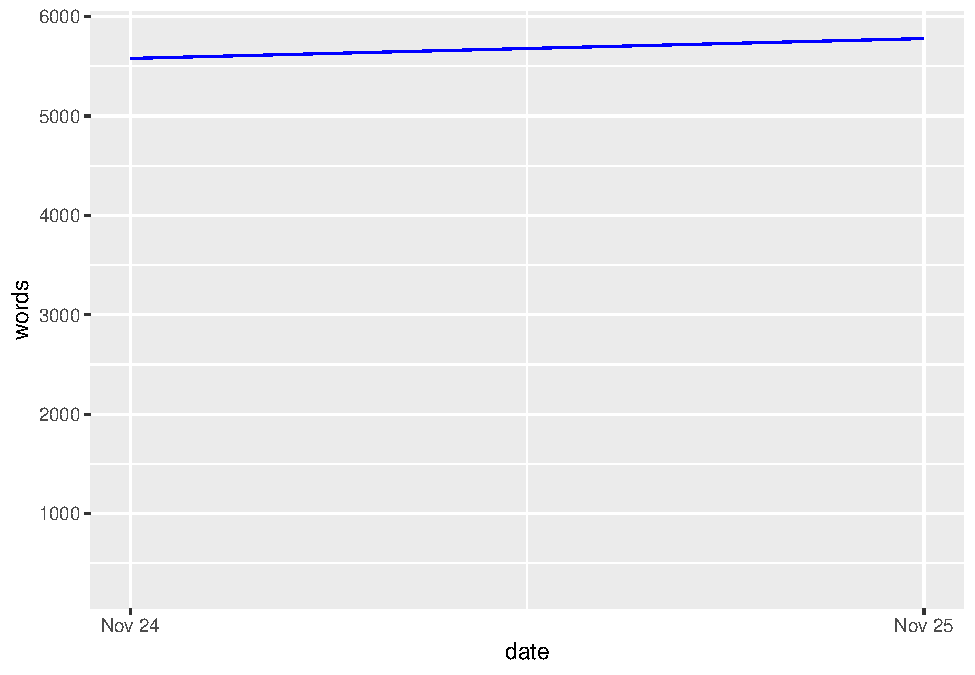
\includegraphics{_main_files/figure-latex/word-count-fig-1.pdf}

\begin{savequote}
Hold
\qauthor{--- Hold}\end{savequote}



\hypertarget{intro-heading}{%
\chapter{Introduction}\label{intro-heading}}

\minitoc 

First I provide a background to the central concepts and themes of this thesis, and justify the motivations for this piece of work. I introduce a tool that allows for systematic searching of preprint literature, which is then used in a systematic review of all available evidence on my central research question.

\hypertarget{additional-ideas}{%
\section{Additional ideas}\label{additional-ideas}}

\begin{itemize}
\tightlist
\item
  Explore difference/similarities between the published and unpublished literature, potentially formally, using funnel plots and also by following up preprints to see if they are eventually published. Limit to the date we ran the original search and see if any study included in the study had not been published by the time the review was finished.
\item
  Compare and contrast the codes used to find the AzD cases in the previous study and in this study, potentially with a view to contrasting misclassification between the two.
\end{itemize}

\hypertarget{aims-and-objectives-of-the-thesis}{%
\section{Aims and Objectives of the thesis}\label{aims-and-objectives-of-the-thesis}}

\hypertarget{aim}{%
\subsection{Aim}\label{aim}}

\hypertarget{objectives}{%
\subsection{Objectives}\label{objectives}}

\begin{itemize}
\tightlist
\item
  To review the published literature with respect to the effec tof lipids and lipid regulating agents\\
\item
  To examine whether there is evidence for an effect of lipid-regulating agents on dementia and related outcomes in a large scale population-based cohort, the Clinical Practice Research Datalink
\item
  To meta-analyze the
\end{itemize}

\hypertarget{theoretical-framework}{%
\section{Theoretical framework}\label{theoretical-framework}}

The main theoretical framework used in this thesis is evidence synthesis - the discovery and critical integration of all available evidence on a research question in order to either: a) provide a more definitive answer to that question or; b) highlight gaps in the existing evidence base, so that future research address questions that have yet to be answered, or explores the same question in a way that increases our confidence in the result.

All elements of this thesis are based around this framework.

\hypertarget{chapter-overview}{%
\section{Chapter Overview}\label{chapter-overview}}

\begin{itemize}
\tightlist
\item
  \textbf{Chapter \ref{background-heading}:} Background information on dementia and blood lipid levels. This chapter provides an introduction to the topics covered in this thesis to non-subject area experts, and discusses the motivation for the remainder of the thesis.
\item
  \textbf{Chapter \ref{sys-rev-tools-heading}} This CHhapter introduces a new tool, the \texttt{medrxivr} R package, which was used to developed to allow for systematic searches of the bioRxiv and medRxiv preprint repositories.
\item
  \textbf{Chapter \ref{sys-rev-heading}} This Chapter describes a comprehensive systematic review and meta-analysis of all available evidence on the relationship between blood lipids and lipid.
\item
  \textbf{Chapter \ref{cprd-analysis-heading}:} This Chapter examines the relationship between lipid-regulating agent use and dementia outcomes in the Clinical Practice Research Datalink, a large primary care electronic health record database, based in England.
\item
  \textbf{Chapter \ref{ipd-heading}:} This Chapter describes an individual patient data analysis of several longitudinal cohort studies, to describe the relationship between blood serum lipids and dementia outcomes.
\end{itemize}

\hypertarget{thesis-output}{%
\section{Thesis Output}\label{thesis-output}}

The outputs of this thesis are detailed below, and include published peer review papers, presentations at conferences, open source evidence synthesis tools, and . . .

\hypertarget{peer-reviewed-papers}{%
\subsection{Peer reviewed papers}\label{peer-reviewed-papers}}

\textbf{Include other papers I have been involved in?}

\begin{itemize}
\item
  McGuinness, Luke A., and Lena Schmidt. ``medrxivr: Accessing and searching medRxiv and bioRxiv preprint data in R.'' Journal of Open Source Software 5.54 (2020): 2651. DOI: \href{https://doi.org/10.21105/joss.02651}{10.21105/joss.02651}
\item
  McGuinness, Luke A., and Julian PT Higgins. ``Risk‐of‐bias VISualization (robvis): An R package and Shiny web app for visualizing risk‐of‐bias assessments.'' Research Synthesis Methods (2020). DOI: \href{https://doi.org/10.1002/jrsm.1411}{10.1002/jrsm.1411}
\end{itemize}

\hypertarget{papers-under-reviewpreprints}{%
\subsection{Papers under review/Preprints}\label{papers-under-reviewpreprints}}

\begin{itemize}
\tightlist
\item
\end{itemize}

\hypertarget{software}{%
\subsection{Software}\label{software}}

\begin{itemize}
\item
  \texttt{medrxvir}: An R package and associated \texttt{shiny} web application that allows users to easily search and retrieve bibliographic data from the medRxiv\footnote{\url{https://www.medrxiv.org/}} and bioRxiv\footnote{\url{https://www.biorxiv.org/}} preprint repositories. See Chapter \ref{sys-rev-tools-heading} for more details. Install a stable version of the package from CRAN with \texttt{install.packages("medrxivr")} or alternatively install the development version from GitHub using \texttt{devtools::install\_github("mcguinlu/medrxivr")}. Link: \url{https://ropensci.github.io/medrxivr/}
\item
  \texttt{robvis}: An R package and associated \texttt{shiny} web application that allows users to easily visualize the results of the risk-of-bias assessments performed as part of a systematic review. See Appendix \ref{appendix-robvis} for more details. Install a stable version of the package from CRAN using \texttt{install.packages("robvis")} or alternatively install the development version from GitHub using \texttt{devtools::install\_github("mcguinlu/robvis")}. Link: \url{https://mcguinlu.github.io/robvis/}
\end{itemize}

\hypertarget{talks}{%
\subsection{Talks}\label{talks}}

\begin{itemize}
\tightlist
\item
  Presentation to the
\item
  Webinar to Evidence Synthesis Ireland on Risk of Bias
\item
  Presentation(s) to the Evidence Synthesis and Meta-Analysis in R Conference (ESMARConf)
\end{itemize}

\hypertarget{peer-review}{%
\subsection{Peer review}\label{peer-review}}

\begin{itemize}
\tightlist
\item
  2 papers for Systematic Reviews
\item
  1 paper for Environment International
\item
  1 paper for Journal of Clinical Epidemiology
\end{itemize}

\hypertarget{summary}{%
\section{Summary}\label{summary}}

\begin{itemize}
\tightlist
\item
\item
\item
\end{itemize}

\begin{savequote}
Science knows it doesn't know everything; otherwise, it'd stop.
\qauthor{--- Dara O'Briain}\end{savequote}



\hypertarget{background-heading}{%
\chapter{Background}\label{background-heading}}

\minitoc 

\hypertarget{lay-summary}{%
\section{Lay summary}\label{lay-summary}}

\hypertarget{introduction}{%
\section{Introduction}\label{introduction}}

\begin{quote}
This chapter provides the context of the thesis. It briefly gives the background on the problem of increased adiposity, the biology of adipose tissue, and diseases linking increased body mass index and mortality. The chapter briefly explores different measures of increased adiposity and potential hypotheses for underlying aetiology of diseases associated with increased adiposity. Finally, the potential application of metabolites and Mendelian randomization in the context of understanding underlying aetiology are discussed. \emph{From Matt Lee's thesis.}
\end{quote}

This Chapter will provide an overview of the key exposures, outcomes and methods used throughout this thesis.

\hypertarget{dementia}{%
\section{Dementia}\label{dementia}}

\hypertarget{definition-and-subtypes}{%
\subsection{Definition and Subtypes}\label{definition-and-subtypes}}

Dementia is major neurocognitive disorder, with symptoms including impairment of executive cognitive functions such as speech, judgement and memory. The most common causes of dementia are Alzheimer's disease and vascular dementia, accounting for \textasciitilde60-80\% and \textasciitilde10\% of cases respectively. The remaining 10-30\% of cases are caused other dementia subtypes (e.g.~Lewy Body dementia) or by progression of other neurological diseases (e.g.~Parkinson's disease).

\hypertarget{diagnosis}{%
\subsection{Diagnosis}\label{diagnosis}}

Dementia is difficult to diagnose, primarily due to the absence of a gold standard test for the condition (is this true, or would it be better to say that there is no gold standard test without an autopsy). Information from multiple diagnostic tools are utilised, from medical history examination, through assessment of patients mental ability (e.g.~the Mini-Mental State Examination), to clinical tests (e.g.~Magnetic Resonance Imaging (MRI) scans).

\hypertarget{criteria}{%
\subsection{Criteria}\label{criteria}}

Several scales are commonly used to diagnose dementia and associated diseases for research purposes. Two of the most commonly used include the criteria of the Diagnostic and Statistical Manual of Mental Disorders, fourth edition (DSM-IV-TR)1 and the National Institute of Neurological Disorders and Stroke--Alzheimer Disease and Related Disorders (NINCDS--ADRDA).\textsuperscript{\protect\hyperlink{ref-dubois2007}{1}} {[}\textbf{Need first NINCDS-ADRDA citation and DSM- }{]}

\textbf{Note important differences between the scales and whether they affect results. Could cross-reference with an exploratory analysis in Chapter \ref{sys-rev-heading}}

\hypertarget{public-health-importance}{%
\subsection{Public Health Importance}\label{public-health-importance}}

Dementia is quickly becoming a critically important public health issue. Despite the age-specific incidence and prevalence of dementia remaining relatively constant over time,6 an ageing population looks set to create a dementia epidemic, particularly in Westernised countries. In the UK, there are estimated to be 800,000 people currently living with dementia, with this figure expected to double by 2040.7 Globally, the prevalence of dementia is expected to reach 75 million by 2030.8 Despite the number of dementia cases and decades of research, there remains much unknown about the pathogenesis and progression of the disease.

\begin{Shaded}
\begin{Highlighting}[]
\FunctionTok{library}\NormalTok{(gt)}
\FunctionTok{library}\NormalTok{(dplyr)}

\FunctionTok{gt}\NormalTok{(}\AttributeTok{data =}\NormalTok{ mtcars) }\SpecialCharTok{\%\textgreater{}\%}
  \FunctionTok{tab\_style}\NormalTok{(}
    \AttributeTok{style =} \FunctionTok{cell\_text}\NormalTok{(}\AttributeTok{weight =} \StringTok{"bold"}\NormalTok{),}
    \AttributeTok{locations =} \FunctionTok{list}\NormalTok{(}\FunctionTok{cells\_body}\NormalTok{(}
      \AttributeTok{columns =} \FunctionTok{vars}\NormalTok{(mpg)),}
      \FunctionTok{cells\_column\_labels}\NormalTok{(}\AttributeTok{columns =} \FunctionTok{vars}\NormalTok{(mpg))))}
\end{Highlighting}
\end{Shaded}

\captionsetup[table]{labelformat=empty,skip=1pt}
\begin{longtable}{rrrrrrrrrrr}
\toprule
mpg & cyl & disp & hp & drat & wt & qsec & vs & am & gear & carb \\ 
\midrule
21.0 & 6 & 160.0 & 110 & 3.90 & 2.620 & 16.46 & 0 & 1 & 4 & 4 \\ 
21.0 & 6 & 160.0 & 110 & 3.90 & 2.875 & 17.02 & 0 & 1 & 4 & 4 \\ 
22.8 & 4 & 108.0 & 93 & 3.85 & 2.320 & 18.61 & 1 & 1 & 4 & 1 \\ 
21.4 & 6 & 258.0 & 110 & 3.08 & 3.215 & 19.44 & 1 & 0 & 3 & 1 \\ 
18.7 & 8 & 360.0 & 175 & 3.15 & 3.440 & 17.02 & 0 & 0 & 3 & 2 \\ 
18.1 & 6 & 225.0 & 105 & 2.76 & 3.460 & 20.22 & 1 & 0 & 3 & 1 \\ 
14.3 & 8 & 360.0 & 245 & 3.21 & 3.570 & 15.84 & 0 & 0 & 3 & 4 \\ 
24.4 & 4 & 146.7 & 62 & 3.69 & 3.190 & 20.00 & 1 & 0 & 4 & 2 \\ 
22.8 & 4 & 140.8 & 95 & 3.92 & 3.150 & 22.90 & 1 & 0 & 4 & 2 \\ 
19.2 & 6 & 167.6 & 123 & 3.92 & 3.440 & 18.30 & 1 & 0 & 4 & 4 \\ 
17.8 & 6 & 167.6 & 123 & 3.92 & 3.440 & 18.90 & 1 & 0 & 4 & 4 \\ 
16.4 & 8 & 275.8 & 180 & 3.07 & 4.070 & 17.40 & 0 & 0 & 3 & 3 \\ 
17.3 & 8 & 275.8 & 180 & 3.07 & 3.730 & 17.60 & 0 & 0 & 3 & 3 \\ 
15.2 & 8 & 275.8 & 180 & 3.07 & 3.780 & 18.00 & 0 & 0 & 3 & 3 \\ 
10.4 & 8 & 472.0 & 205 & 2.93 & 5.250 & 17.98 & 0 & 0 & 3 & 4 \\ 
10.4 & 8 & 460.0 & 215 & 3.00 & 5.424 & 17.82 & 0 & 0 & 3 & 4 \\ 
14.7 & 8 & 440.0 & 230 & 3.23 & 5.345 & 17.42 & 0 & 0 & 3 & 4 \\ 
32.4 & 4 & 78.7 & 66 & 4.08 & 2.200 & 19.47 & 1 & 1 & 4 & 1 \\ 
30.4 & 4 & 75.7 & 52 & 4.93 & 1.615 & 18.52 & 1 & 1 & 4 & 2 \\ 
33.9 & 4 & 71.1 & 65 & 4.22 & 1.835 & 19.90 & 1 & 1 & 4 & 1 \\ 
21.5 & 4 & 120.1 & 97 & 3.70 & 2.465 & 20.01 & 1 & 0 & 3 & 1 \\ 
15.5 & 8 & 318.0 & 150 & 2.76 & 3.520 & 16.87 & 0 & 0 & 3 & 2 \\ 
15.2 & 8 & 304.0 & 150 & 3.15 & 3.435 & 17.30 & 0 & 0 & 3 & 2 \\ 
13.3 & 8 & 350.0 & 245 & 3.73 & 3.840 & 15.41 & 0 & 0 & 3 & 4 \\ 
19.2 & 8 & 400.0 & 175 & 3.08 & 3.845 & 17.05 & 0 & 0 & 3 & 2 \\ 
27.3 & 4 & 79.0 & 66 & 4.08 & 1.935 & 18.90 & 1 & 1 & 4 & 1 \\ 
26.0 & 4 & 120.3 & 91 & 4.43 & 2.140 & 16.70 & 0 & 1 & 5 & 2 \\ 
30.4 & 4 & 95.1 & 113 & 3.77 & 1.513 & 16.90 & 1 & 1 & 5 & 2 \\ 
15.8 & 8 & 351.0 & 264 & 4.22 & 3.170 & 14.50 & 0 & 1 & 5 & 4 \\ 
19.7 & 6 & 145.0 & 175 & 3.62 & 2.770 & 15.50 & 0 & 1 & 5 & 6 \\ 
15.0 & 8 & 301.0 & 335 & 3.54 & 3.570 & 14.60 & 0 & 1 & 5 & 8 \\ 
21.4 & 4 & 121.0 & 109 & 4.11 & 2.780 & 18.60 & 1 & 1 & 4 & 2 \\ 
\bottomrule
\end{longtable}

\hypertarget{challenges-in-the-study-of-dementia-using-traditional-study-designs}{%
\subsection{Challenges in the study of dementia using traditional study designs}\label{challenges-in-the-study-of-dementia-using-traditional-study-designs}}

Speak to the

Historically, studies on dementia have faced a range of challenges. As a range of determinants (genetic, environmental and lifestyle) are thought to jointly influence the risk, progression and outcomes of dementia, any individual association is likely to have only a small effect. Therefore, the statistical power need to detect these associations will often require sample sizes that are unfeasible using primary data collection.
This fact is further complicated by the long latency of dementia, which necessitates a costly long-term approach to patient follow-up. Furthermore, dementia studies often have limited generalisability to the target population, as certain subgroups (e.g.~the very old) are frequently under-represented in study cohorts due to difficulties associated with their recruitment.9 Finally, studies employing a case-control design are further limited by the high potential for differential recall bias between those who have and have not developed dementia.10

Fortunately, these limitations may potentially be addressed through the use of routinely collected health data, and the electronic health record databases in which they are stored.

\emph{Cognitive impairment not dementia} (CIND) is another term used to described those with cognitivie impairment but who fall below the diagnostic criteria for dementia.

A further clinical subtype that is of particular import the

And MCI

And different scales

\hypertarget{history}{%
\subsection{History}\label{history}}

\begin{quote}
Two major clinical trials are often cited as providing evidence that statins do not have an effect on the incidence ofdementia: the Prospective Study ofPravastatin in the Elderly (PROSPER) and the Medical Research
Council/British Heart Foundation Heart Protection Study; however, because of methodologic limitations in relation to dementia outcomes in these two trials, the results of these trials are difficult to evaluate. Dementia incidence or cognitive outcomes were not preplanned endpoints in either of them, neither study included a clinical cognitive evaluation, and numbers of patients with follow-up information for cognitive evaluations were not reported in either study manuscript. In PROSPER a post hoc analysis compared changes in cognitive scores over a 3-year period between statintreated and placebo patients and found no significant differences. In the MRC/BHF HPS trial,27
similar percentages of participants (0.3\% in each---statin vs placebo---group) developed dementia during the 5-year follow-up period. The report did not state how the outcome of dementia was determined (e.g., reported as an adverse event or by follow-up phone interview).
\emph{Taken from Cramer 2008 - included in review}
\end{quote}

There exist only two large scale randomized controlled trials - in fact these studies are the only two trials included in a 2016 review of statins for the prevention of dementia produced by the Cochrane.\textsuperscript{\protect\hyperlink{ref-mcguinness2016b}{2}} Both showed no effect of

Queries around how the data were collected, along

\hypertarget{economic-impact}{%
\subsection{Economic impact}\label{economic-impact}}

\hypertarget{risk-factors}{%
\subsection{Risk factors}\label{risk-factors}}

\hypertarget{treatments}{%
\subsection{Treatments}\label{treatments}}

\hypertarget{preventative-measures}{%
\subsection{Preventative measures}\label{preventative-measures}}

\hypertarget{serum-lipids}{%
\section{Serum lipids}\label{serum-lipids}}

\hypertarget{range-of-lipids}{%
\subsection{Range of lipids}\label{range-of-lipids}}

The blood profile has a range of lipid fractions to it. However, for the sake of this thesis, we will only consider the three most important fractions, namely total cholesterol, low density lipoprotein cholesterol (LDLc), high density lipoprotein cholesterol (HDLc) and trigylcerides (TG).

\hypertarget{hdl-c}{%
\subsection{HDL-c}\label{hdl-c}}

\hypertarget{ldl-c}{%
\subsection{LDL-c}\label{ldl-c}}

Include formula for working out total cholesterol and the ranges.

LDL-c levels are not directly measured but instead are estimated from using the Friedewald formula,\textsuperscript{\protect\hyperlink{ref-friedewald1972}{3}} where the :

\[LDLc \approx TC - HDLc - kTG\]
where \(k\) is 0.20 if measurements are in mg/dl and 0.45 if in mmol/l.

Limitations to the method include a requirement to fast for 12-14hrs prior to measures, an inability to estimate LDLc if TG levels are high

\begin{correction}
Measurement error is a big deal for this thesis, as will discuss
measurement error regarding how different codelists/measurement of AD vs
vascular dementia affect results in later chapters.
\end{correction}

\hypertarget{triglycerides}{%
\subsection{Triglycerides}\label{triglycerides}}

\hypertarget{total-cholesterol}{%
\subsection{Total cholesterol}\label{total-cholesterol}}

\hypertarget{serum-lipid-interventions}{%
\section{Serum lipid interventions}\label{serum-lipid-interventions}}

\hypertarget{statins}{%
\subsection{Statins}\label{statins}}

\hypertarget{lipophilic}{%
\subsubsection{Lipophilic}\label{lipophilic}}

\hypertarget{hydrophilic}{%
\subsubsection{Hydrophilic}\label{hydrophilic}}

\hypertarget{methods-used-in-the-thesis}{%
\section{Methods used in the thesis}\label{methods-used-in-the-thesis}}

\hypertarget{evidence-synthesis}{%
\subsection{Evidence synthesis}\label{evidence-synthesis}}

\hypertarget{primary-cohort-analysis}{%
\subsection{Primary cohort analysis}\label{primary-cohort-analysis}}

\hypertarget{triangulation}{%
\subsection{Triangulation}\label{triangulation}}

\hypertarget{individual-patient-data-meta-analyis}{%
\subsection{Individual patient data meta-analyis}\label{individual-patient-data-meta-analyis}}

\hypertarget{summary-1}{%
\section{Summary}\label{summary-1}}

\begin{savequote}
Why are open source statistical programming\\
languages the best?

Because they R.
\qauthor{--- Bealy, 2013\textsuperscript{\protect\hyperlink{ref-bealy2013}{4}}}\end{savequote}



\hypertarget{sys-rev-tools-heading}{%
\chapter{medrxivr: an R package for systematically searching biomedical preprints}\label{sys-rev-tools-heading}}

\minitoc 

\hypertarget{main-points-to-be-removed}{%
\section{Main points (to be removed)}\label{main-points-to-be-removed}}

The main points I want to get across in this Chapter are:

\begin{itemize}
\item
  Why searching preprints is important
\item
  Why existing methods are not sufficient
\item
  What the \texttt{medrxivr} tool adds
\end{itemize}

\hypertarget{lay-summary-1}{%
\section{Lay summary}\label{lay-summary-1}}

Preprints are copies of academic manuscripts that are posted online in advance of being formally published by an academic journal. They represent an important source of scientific literature. A new software program called \texttt{medrxivr} was created to allow researchers to find preprints related to their research in a transparent and reproducible way. Development of this tool was an essential part of this thesis, as preprints represent a key source of information needed for the research reported in future chapters.

\hypertarget{introduction-1}{%
\section{Introduction}\label{introduction-1}}

Preprints represent an increasingly important source of scientific information. Defined by the Committee on Publication Ethics (COPE) as `scholarly manuscript{[}s{]} posted by the author(s) in an openly accessible platform, usually before or in parallel with the peer review process'\textsuperscript{\protect\hyperlink{ref-committeeonpublicationethicscope2018}{5}}, preprints serve several purposes. They are used to establish primacy when submitting to a journal where the peer-review process may take several months;\textsuperscript{\protect\hyperlink{ref-vale2016}{6}} to rapidly disseminate research findings, as occurred during the COVID-19 pandemic;\textsuperscript{\protect\hyperlink{ref-fraser2020a}{7}} and to make available publications that may not have been accepted elsewhere in an attempt to combat publication bias or the ``file-drawer'' effect.\textsuperscript{\protect\hyperlink{ref-rosenthal1979}{8}}

As a result, repositories of preprinted articles should be considered a distinct but complementary information source when reviewing the evidence base as part of a systematic review. The two key repositories in the health science are bioRxiv, established in 2013,\textsuperscript{\protect\hyperlink{ref-sever2019}{9}} and medRxiv, which evolved to replace the ``Epidemiology'' and ``Clinical Trial'' categories of bioRxiv, which launched in 2019.\textsuperscript{\protect\hyperlink{ref-rawlinson2019}{10}}

Searching these preprints as part of the systematic review described in Chapter \ref{sys-rev-heading} was a necessity, as many of the existing reviews on the topic of lipids and dementia have not considered this important source of grey literature. At the time of writing, however, the bioRxiv.medRxiv websites allow only simple search queries as opposed to the often complex Boolean logic (AND/OR/NOT) that information specialists use to query other major databases.{[}@bramer2018a;@gusenbauer2020{]} Additionally, the best available extraction mechanism for obtaining references for all records returned by a search were to go through each record, one-by-one, downloading individual citations. As the scale of these preprint databases increase, particularly in light of the massive expansion of the medRxiv repository as a result of COVID, this already time-consuming and error-prone method is no longer feasible.

This chapter outlines the development and key functionality of \texttt{medrxivr} (version 0.0.5), a tool created to facilitate the searching of medRxiv and bioRxiv preprints. The factors that necessitated the development of this tool in the context of this thesis are outlined, and the use of \texttt{medrxivr} in external projects and by other researchers is discussed. As the majority of work on this aspect of this thesis is represented by lines of code, this Chapter is a high-level summary of the work done on this project. The GitHub repository\footnote{Available at \url{https://github.com/ropensci/medrxivr}} for the \texttt{medrxivr} contains a complete record of the development of this tool, including discussion with other members of the systematic review community.

~





\begin{figure}
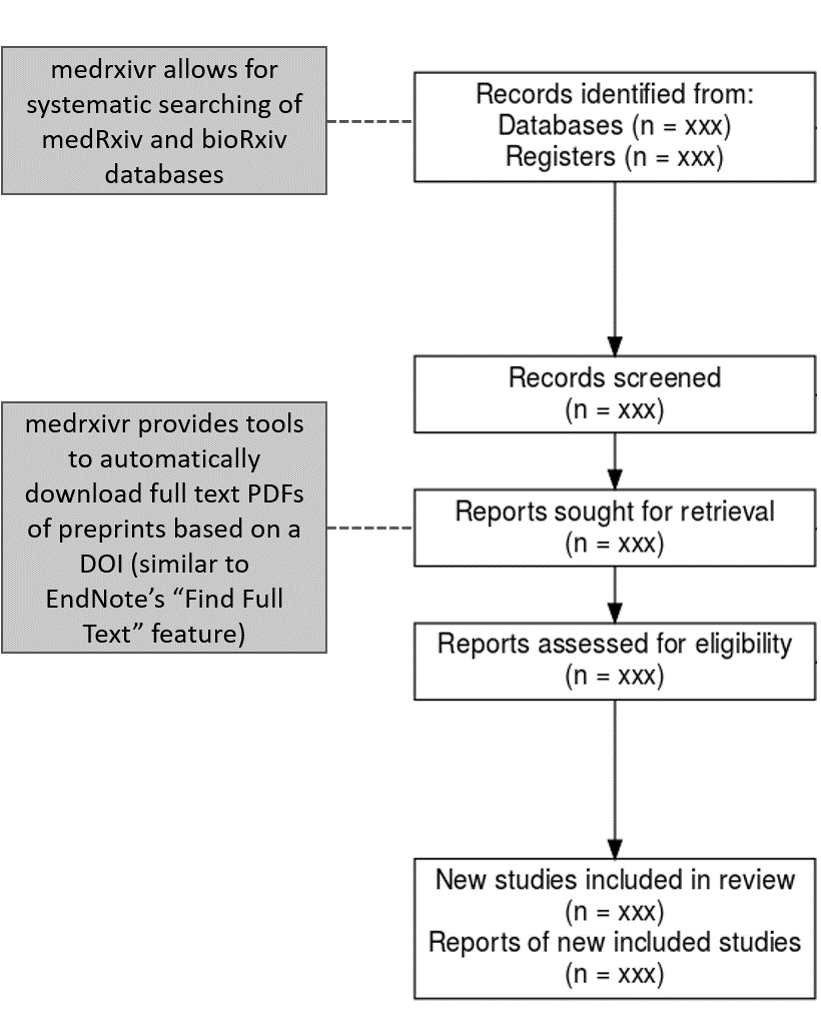
\includegraphics[width=1\linewidth]{figures/sys-rev-tools/medrxiv-role} \caption[Role of \texttt{medrxivr} in a systematic review workflow]{\textbf{Role of \texttt{medrxivr} in a systematic review workflow:} \texttt{medrxivr} allows for systematic searching of biomedical preprints as part of the initial literature searching. Following title and abstract screening, reviewers can then programmatically retrieve a copy of the PDF of included records to facilitate the full-text screening stage (similar to Endnote's ``Find Full Text'' feature).}\label{fig:medrxivr-sr}
\end{figure}

\hypertarget{development}{%
\section{Development}\label{development}}

\hypertarget{success-criteria}{%
\subsection{Success criteria}\label{success-criteria}}

The tool was developed to meet three success criteria,\textsuperscript{\protect\hyperlink{ref-wateridge1995}{11}} influenced both by the functionality required to perform systematic searches as part of the review in Chapter \ref{sys-rev-heading}, discussion with information specialist colleagues, and an informal survey of the evidence synthesis and health librarian communities on Twitter. The criteria were as follows:

\begin{enumerate}
\def\labelenumi{\arabic{enumi}.}
\item
  reliable, reproducible and transparent search functionality, allowing for Boolean (AND/OR/NOT) operator logic;
\item
  support for bulk export of references returned by the search to a file type that can be readily imported into a reference manager (e.g., \emph{.bib} or \emph{.ris}); and
\item
  automated retrieval of the full-text PDFs of relevant records, similar to the Find Full Text feature offered by EndNote.
\end{enumerate}

~

\hypertarget{alternative-medrxivbiorxiv-interfaces}{%
\subsection{Alternative medRxiv/bioRxiv interfaces}\label{alternative-medrxivbiorxiv-interfaces}}

Prior development of this tool, an audit of existing tools for accessing medRxiv and bioRxiv metadata was conducted. While none address the success criteria described above, two of these tools are useful to consider to highlight the additional functionality that \texttt{medrxivr} contributes.

The first, a platform called Rxivist,\textsuperscript{\protect\hyperlink{ref-abdill2019}{12}} allows users to search preprints using keywords. However, the core functionality of the Rxivist platform is focused around exploring the number of times a preprint has been downloaded and/or shared on Twitter, to allow researchers to find the most popular papers related to their topic. The search interface\footnote{Available at \url{https://rxivist.org/}} does not allow for complex search strategies using Boolean operators and there is no option to batch-export the results of a search.

The second tool, \texttt{search.bioPreprint}, allows users to search for terms across a range of preprint servers, including medRxiv and bioRxiv, but also journals which use a post-publication peer-review process such as F1000Research.\textsuperscript{\protect\hyperlink{ref-iwema2016}{13}} However, similar to the Rxivist platform, this tool is designed for researchers aiming to keep up to date with recent developments in their fields rather than systematically assess the entirety of the available literature. As such, the platform only returns the most recent 1,000 records by publication date.

Finally, neither tool provides an easy way to programmatically download a copy of the PDF of relevant preprints as part of the preparation for the full-text screening stage of a systematic review.

~

\hypertarget{early-versions}{%
\subsection{Early versions}\label{early-versions}}

Work on the \texttt{medrxivr} tool began in Summer 2019, and initially consisted of a development of set of R scripts to allow for searching medRxiv and bioRxiv as part of the systematic search outlined in Chapter \ref{sys-rev-heading}. Following interest from other researchers in using the \emph{ad-hoc} web-scraping scripts, additional development work took place in 2019/2020, allowing for improved searching and exporting functionality and the initial version of the \texttt{medrxivr} R package was released in February 2020.

Early versions of the tool had a reliance on scraping data directly from the repository website. Web-scraping is a fragile mechanism for extracting data, as it is entirely dependent on consistent website design and underlying code structure remaining unchanged.\textsuperscript{\protect\hyperlink{ref-shaw2002}{14},\protect\hyperlink{ref-laprie1992}{15}}. In the case of \texttt{medrxivr}, constant maintenance work was required to ensure the web-scraping script performed as expected, as the repository website was regularly updated.

However, an Application Programming Interface (API) for the medRxiv and bioRxiv repositories was made public in early 2020 by the institution responsible for managing these preprint repositories, the Cold Springs Harbor Laboratory. This allowed for newer versions of the \texttt{medrxivr} package to engage in active ``fault prevention'' and provide a more robust interface to the data by removing the reliance of web-scraping.\textsuperscript{\protect\hyperlink{ref-laprie1992}{15}}

\hypertarget{package-infrastructure}{%
\subsection{Package infrastructure}\label{package-infrastructure}}

The \texttt{medrxvir} package was written in R using RStudio,\textsuperscript{\protect\hyperlink{ref-rcoreteam2019}{16}} and followed development best-practice, including detailed documentation, a robust unit testing framework (99\% of all code lines within the package are formally tested across multiple platforms including Windows, MacOS, and Linux), and in-depth code review by two experienced, independent reviewers.

~

\hypertarget{usage}{%
\section{Usage}\label{usage}}

The \texttt{medrxivr} R package is split into two component parts:

\begin{itemize}
\tightlist
\item
  an interface to the Cold Springs Harbor Laboratory API, which imports medRxiv and bioRxiv metadata into R; and
\item
  a collection of functions for working with the imported metadata, with an explicit focus on searching this data as part of a systematic review or evidence synthesis project.
\end{itemize}

The standard workflow is to download a copy of all metadata contained in the repository, and then to perform searches on this local copy. This is a workaround as the Cold Springs Harbor Laboratory API does not provide any functionality to search the database.

While the package allows for users to search both medRxiv and bioRxiv, as the process is identical for both, the examples in the sections are limited to the medRxiv repository.

~

\hypertarget{installation}{%
\subsection{Installation}\label{installation}}

\texttt{medrxivr} has been released to the Comprehensive R Archive Network (CRAN), and can be installed with the following code:

~

\begin{Shaded}
\begin{Highlighting}[]
\FunctionTok{install.packages}\NormalTok{(}\StringTok{"medrxivr"}\NormalTok{)}
\end{Highlighting}
\end{Shaded}

~

Alternatively, the development version of the package can be installed from GitHub:

~

\begin{Shaded}
\begin{Highlighting}[]
\CommentTok{\# install.packages("devtools") }
\NormalTok{devtools}\SpecialCharTok{::}\FunctionTok{install\_github}\NormalTok{(}\StringTok{"ropensci/medrxivr"}\NormalTok{)}
\end{Highlighting}
\end{Shaded}

~

\hypertarget{importing-preprint-metadata}{%
\subsection{Importing preprint metadata}\label{importing-preprint-metadata}}

\texttt{medrixvr} provides two ways to access medRxiv data. The first, via the \texttt{mx\_api\_content()} function, creates a local copy of all data available from the medRxiv API at the time the function is run.

~

\begin{Shaded}
\begin{Highlighting}[]
\CommentTok{\# Get a copy of the database from the live medRxiv API endpoint}
\NormalTok{mx\_data }\OtherTok{\textless{}{-}} \FunctionTok{mx\_api\_content}\NormalTok{()  }
\end{Highlighting}
\end{Shaded}

~

The second, via the \texttt{mx\_snapshot()} function, provides access to a maintained static snapshot of the database, created each morning at 6am using \texttt{mx\_api\_content()}. Allowing users of \texttt{medrxivr} to access a maintained snapshot removes any dependency on the API, which can become unavailable during peak usage times. The relationship between the two methods for accessing the data contained in the medRxiv database is summarized in Figure \ref{fig:medrxivr-data-sources}.

~

\begin{Shaded}
\begin{Highlighting}[]
\CommentTok{\# Import a copy of the medRxiv data from the snapshot}
\NormalTok{mx\_data }\OtherTok{\textless{}{-}} \FunctionTok{mx\_snapshot}\NormalTok{()}
\end{Highlighting}
\end{Shaded}

~





\begin{figure}[!h]
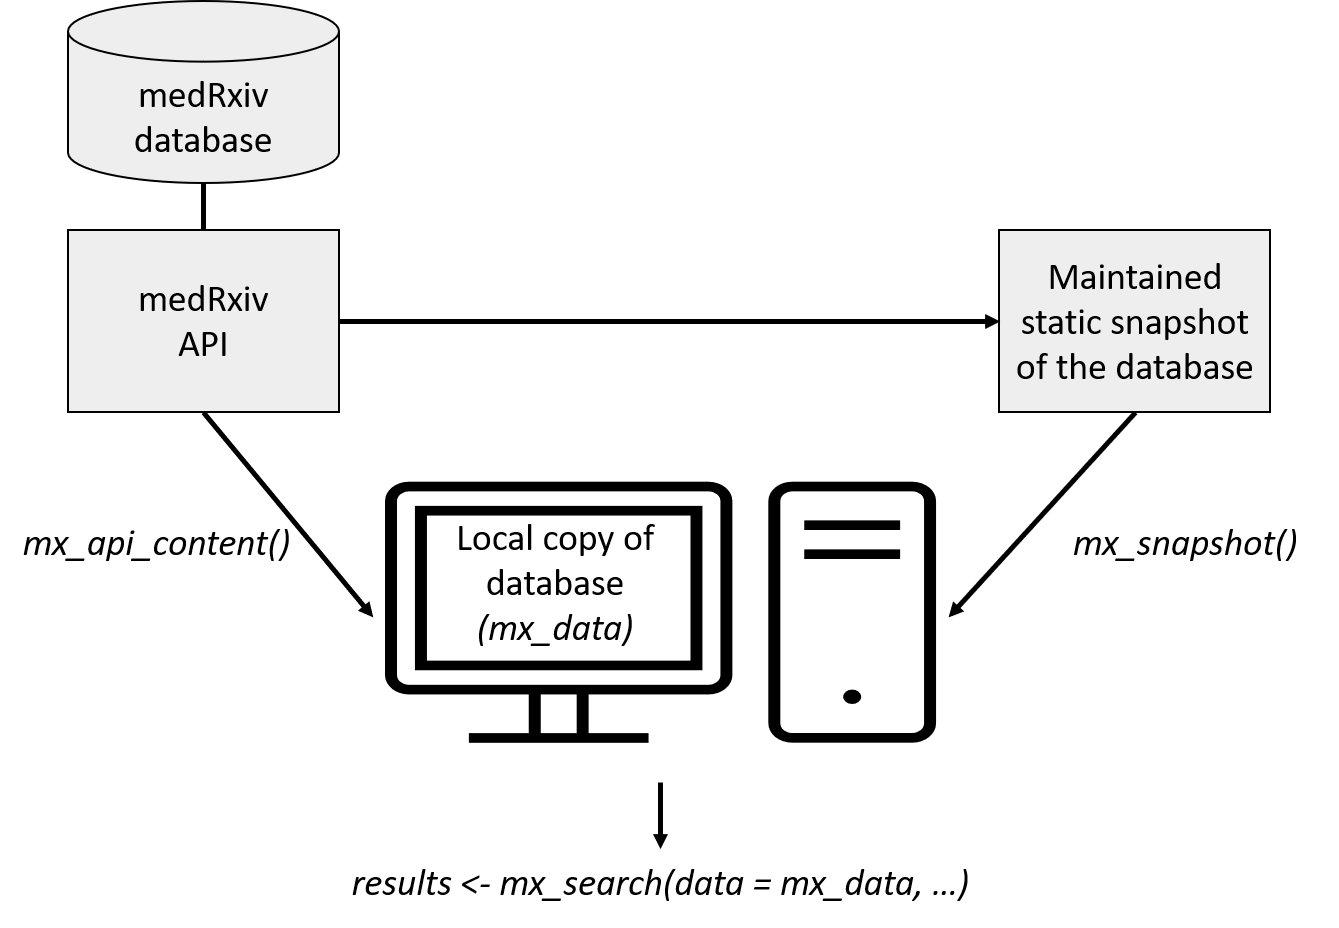
\includegraphics[width=1\linewidth]{figures/sys-rev-tools/data_sources} \caption[Overview of \texttt{medrxivr} data sources]{\textbf{Overview of \texttt{medrxivr} data sources:} Users can either access the API directly via \texttt{mx-api\_content()}, or can import a maintained snapshot of the database, taken each morning at 6am, via the \texttt{mx\_snapshot()} function. Note: due to the size of bioRxiv, only a maintained snapshot of the medRxiv repository is available via \texttt{mx\_snapshot()}.}\label{fig:medrxivr-data-sources}
\end{figure}

~

\hypertarget{performing-a-search}{%
\subsection{Performing a search}\label{performing-a-search}}

Once a local copy of the metadata is created, the first step in searching it is to create a search strategy. Search terms to be combined with the OR operator are contained in vectors (\texttt{c(...)}), while topics to be combined with the AND operator are contained in lists (\texttt{list(\ldots{})}).

~

\begin{Shaded}
\begin{Highlighting}[]
\CommentTok{\# Create the search query}
\NormalTok{topic1  }\OtherTok{\textless{}{-}} \FunctionTok{c}\NormalTok{(}\StringTok{"dementia"}\NormalTok{,}\StringTok{"alzheimer\textquotesingle{}s"}\NormalTok{)  }\CommentTok{\# Combined with OR}
\NormalTok{topic2  }\OtherTok{\textless{}{-}} \FunctionTok{c}\NormalTok{(}\StringTok{"lipids"}\NormalTok{,}\StringTok{"statins"}\NormalTok{)        }\CommentTok{\# Combined with OR}

\NormalTok{myquery }\OtherTok{\textless{}{-}} \FunctionTok{list}\NormalTok{(topic1, topic2)         }\CommentTok{\# Combined with AND}
\end{Highlighting}
\end{Shaded}

~

For example, when written in standard syntax, the search contained in the \texttt{myquery} object above would be: ``((dementia \textbf{OR} alzheimer's) \textbf{AND} (lipids \textbf{OR} statins))''. There is now limit to the number of search terms that can be included in each topic, nor in the number of topics that can be search for. Search terms can also contain common syntax used by systematic reviewers and health librarians, including the use of NEAR statements which allows for identification of co-localised terms, and wild-cards, which allow for alternate spellings, e.g.~``randomi\emph{s}ation'' vs ``randomi\emph{z}ation''.

Once a strategy has been defined, it is passed along with the local copy of the database to the \texttt{mx\_search()} function.

~

\begin{Shaded}
\begin{Highlighting}[]
\CommentTok{\# Run the search}
\NormalTok{results }\OtherTok{\textless{}{-}} \FunctionTok{mx\_search}\NormalTok{(mx\_data,}
\NormalTok{                     myquery)}
\end{Highlighting}
\end{Shaded}

~

\hypertarget{refining-your-search}{%
\subsection{Refining your search}\label{refining-your-search}}

An important argument of the \texttt{mx\_search()} is \texttt{report}, which outputs a structured table with each search strategy presented on an individual line and the number of records associated with this strategy.

~

\begin{Shaded}
\begin{Highlighting}[]
\NormalTok{results  }\OtherTok{\textless{}{-}} \FunctionTok{mx\_search}\NormalTok{(mx\_data,}
                      \FunctionTok{c}\NormalTok{(}\StringTok{"dementia"}\NormalTok{, }\StringTok{"alzheimer\textquotesingle{}s"}\NormalTok{), }\CommentTok{\# Combined with OR}
                      \AttributeTok{report =} \ConstantTok{TRUE}\NormalTok{)}
\end{Highlighting}
\end{Shaded}

\begin{Shaded}
\begin{Highlighting}[]
\DocumentationTok{\#\# Found 203 record(s) matching your search.}
\DocumentationTok{\#\# Total topic 1 records: 203}
\DocumentationTok{\#\# dementia: 203}
\DocumentationTok{\#\# Total topic 2 records: 0}
\DocumentationTok{\#\# alzheimer’s: 0}
\end{Highlighting}
\end{Shaded}

~

This allows users to discover which terms in their search are contributing most to the total number of results returned. This is important as part of developing a search strategy,\textsuperscript{\protect\hyperlink{ref-bramer2018}{17}} as it allows for the key terms related to each topic to be discovered. It also aids in identifying misspelled search terms, which will frequently return no results.

~

\hypertarget{exporting-to-a-bibliography-file}{%
\subsection{Exporting to a bibliography file}\label{exporting-to-a-bibliography-file}}

In line with the second success criteria (Section \ref{success-criteria}), one of the key features of the \texttt{medrxivr} is the ability for users to easily export the results of their systematic search to a reference manager. While it is a seemingly simple request, this is is one of the key ways in which \texttt{medrxivr} is set apart for other preprint search tools, including the native medRxiv/bioRxiv website search functionality.

For example, the results of our simple search above can be exported to the \texttt{"medrxiv\_export.bib"} file using the following code:

\begin{Shaded}
\begin{Highlighting}[]
\FunctionTok{mx\_export}\NormalTok{(results, }
          \AttributeTok{file =} \StringTok{"medrxiv\_export.bib"}\NormalTok{,}
          \AttributeTok{report =} \ConstantTok{TRUE}\NormalTok{)}
\end{Highlighting}
\end{Shaded}

~

\hypertarget{downloading-the-pdfs-of-relevant-records}{%
\subsection{Downloading the PDFs of relevant records}\label{downloading-the-pdfs-of-relevant-records}}

\texttt{medrxivr} alos allows users to download the full text papers for records that are deemed eligible for full-text screening (see Figure \ref{fig:medrxivr-sr}). \texttt{mx\_download()} takes the list of included records and saves the PDF for each to a folder specified by the user. This functionality is similar to the ``Find Full Text'' feature offered by EndNote.

~

\begin{Shaded}
\begin{Highlighting}[]
\FunctionTok{mx\_download}\NormalTok{(results,  }\CommentTok{\# Search results, less excluded records}
            \StringTok{"pdf/"}\NormalTok{)   }\CommentTok{\# Directory to save PDFs to }
\end{Highlighting}
\end{Shaded}

~

\hypertarget{discussion}{%
\section{Discussion}\label{discussion}}

\hypertarget{reception-and-future-plans}{%
\subsection{Reception and future plans}\label{reception-and-future-plans}}

The tool has be well received by the community (as of March 2021, \texttt{medrxivr} has been downloaded more than 2400 times), and several use cases have been reported. It has been used to visualize the growing number of preprints related to the 2019 coronavirus outbreak,\footnote{\url{https://twitter.com/L_Brierley/status/1233109086444695553}} perform searches of preprints as part of systematic reviews,\textsuperscript{\protect\hyperlink{ref-noone2020}{18}} and examine how data-sharing behaviour is affected by different publication policies (preprint server versus journal).{[}CITE{]}

Following rigorous peer-review, it has been onboarded into the rOpenSci suite of packages, a collection of ``carefully vetted, staff- and community-contributed R software tools that lower barriers to working with scientific data sources on the web'',{[}CITE{]} and an associated article published in the Journal of Open Source Software.\textsuperscript{\protect\hyperlink{ref-mcguinness2020a}{19}} The entire review discussion is publicly available and can be viewed online.\footnote{\url{https://github.com/ropensci/software-review/issues/380}} The tool has also been well received by the open-source community, demonstrated by the engagement of other developers in contributing to important new functionality and suggesting bug-fixes.

{[}Add bit about the benefits of the rOpenSci review process{]}

Lobbying of the Cold Springs Harbor Laboratory to develop the API to allow for direct searching of the database has been ongoing. This would negate the current need to download a local copy of the relevant preprint database before searching it, which is currently the rate limiting step for performing searches. For example, as of January 2021, downloading a copy of the bioRxiv database takes approximately an hour.

~

\hypertarget{limitations-of-medrxivr}{%
\subsection{\texorpdfstring{Limitations of \texttt{medrxivr}}{Limitations of medrxivr}}\label{limitations-of-medrxivr}}

While searching of the medRxiv and bioRxiv databases was crucial for the systematic review element of this thesis presented in Chapter \ref{sys-rev-heading}, there are some important limitations to note here. A key example is that the tool only searches the available metadata of preprint records (the title, abstract and keywords), rather than the full text of preprints, meaning some relevant records might be missed. However, this approach ethos other search platforms such as OvidSP, and while some relevant records may be missed (reduced sensitivity), limiting the search to the metadata fields prevents non-relevant records from being returned (high specificity). A key example of the reduced specificity when searching the full text, identified during development of \texttt{medrxivr}, is that a search for ``dementia'' would return a record where the only occurrence of this term is in the title of one of the references.\textsuperscript{\protect\hyperlink{ref-bong2019}{20}}

There is also the potential that the cross-section of literature posted on medrxiv/bioRxiv would be substantially different from the true grey literature (studies or analyses that are not published for a range of reasons including results that are not deemed ``novel'' or are not statistically significant).\textsuperscript{\protect\hyperlink{ref-song2010}{21}} This is because simply lowering the barriers to publication may well encourage authors to published ``null'' results, but due to the effort involved in writing up a distributable manuscript, it is unlikely to completely address the ``file drawer'' effect.\textsuperscript{\protect\hyperlink{ref-rosenthal1979}{8}} It is likely too early (and likely too methodologically difficult) to tell whether the increased popularity and acceptance of preprint repositories will have any effect of the availability of research that was not considered ``publishable'' at other venues. (This disagress with the use cases listed in the intro!)

~

\hypertarget{role-of-open-source-tools-in-evidence-synthesis}{%
\subsection{Role of open source tools in evidence synthesis}\label{role-of-open-source-tools-in-evidence-synthesis}}

\emph{Not sure where this should go, but keen to include it}

Part of the motivation for creating the \texttt{medrxivr} tool was a belief that the development and distribution of open source scripts and tools should be a fundamental part of evidence synthesis research.\textsuperscript{\protect\hyperlink{ref-goldacre2019b}{22},\protect\hyperlink{ref-mckiernan2016c}{23}} In the case of \texttt{medrxivr}, it is likely that several other evidence synthesists had written personal scripts that have a similar, or related, functionality - in fact, following development of the tool, I identified one other researcher that has done so (Nicholas Fraser, author of the \texttt{rbiorxiv} package, which allows for importing medRxiv metadata into R but does not provide search functionality).\textsuperscript{\protect\hyperlink{ref-rbiorxiv}{24}} If these scripts continue to be developed in private and are never shared or publicised, this will inevitably lead to harm to the evidence synthesis community, not only in terms of duplication of time and effort but also due to lost opportunities for collaboration.\textsuperscript{\protect\hyperlink{ref-mckiernan2016c}{23}} Creating and sharing well-documented packages, the recognised standard for sharing code in R, represents one way to reduce this inefficiency.\textsuperscript{\protect\hyperlink{ref-vuorre2020}{25}}

\hypertarget{summary-2}{%
\section{Summary}\label{summary-2}}

\begin{itemize}
\item
  In this Chapter, I have introduced a new tool, \texttt{medrxivr}, for performing complex systematic searches of the medRxiv and bioRxiv preprint repositories.
\item
  I have outlined the motivation for developing this tool in relation to this thesis - more specifically, that it was used to perform systematic and reproducible searches of a key literature sources used in the comprehensive systematic review described in Chapter \ref{sys-rev-heading}.
\item
  I have contrasted \texttt{medrxivr} with other available interfaces to medRxiv/bioRxiv data to highlight the added functionality it offers. I have also discussed the tools reception to date, a roadmap for its future development and its place in the broader evidence synthesis in R ecosystem.
\end{itemize}

\begin{savequote}
``It is surely a great criticism of our profession that we have not
organised a critical summary by speciality or sub-speciality, up-dated
periodically, of all relevant RCTS.''
\qauthor{--- Archie Cochrane, 2000\textsuperscript{\protect\hyperlink{ref-cochrane20001931}{26}}}\end{savequote}



\hypertarget{sys-rev-heading}{%
\chapter{Systematic review of all available evidence}\label{sys-rev-heading}}

\minitoc 

\hypertarget{to-do}{%
\section{To Do}\label{to-do}}

\begin{itemize}
\tightlist
\item
  Examine how many times a primary study was included in a review\\
\item
  Look at whether searching preprints made any difference to my results
\item
  Could apply ROBIS to previous reviews to see how they stack-up?
\end{itemize}

\hypertarget{lay-summary-2}{%
\section{Lay summary}\label{lay-summary-2}}

\hypertarget{additional-ideas-1}{%
\section{Additional ideas}\label{additional-ideas-1}}

\begin{itemize}
\tightlist
\item
  Evidence map - show the distribution of the different studies population across the world.
\item
  Living systematic review approach - update weekly based on medRxiv
\end{itemize}

\hypertarget{aims}{%
\section{Aims}\label{aims}}

The aim of this chapter is to systematically review all available literature on the association between blood levels of total cholesterol and it's constituent parts (HDL-c,LDL-c and triglycerides) on the subsequent risk of dementia.

Based on the review of prev, no previous

Literature con

\hypertarget{methods}{%
\section{Methods}\label{methods}}

\hypertarget{search-strategy}{%
\subsection{Search strategy}\label{search-strategy}}

We will systematically search electronic bibliographic databases to identify potentially relevant records. The search strategy used in each database will be developed in an iterative manner using a combination of free text and controlled vocabulary (MeSH/EMTREE) terms to identify studies which have examined the relationship between blood lipids levels and dementia, incorporating input from an information specialist. The strategy will include terms related to lipids, lipid modifying treatments, and dementia and its sub-types, and will be designed for MEDLINE before being adapted for use in the other bibliography databases listed. An outline of the general strategy is presented in the Table 3.2 below and the full draft search strategies for each database are attached to this protocol. To ensure that the study design filters are not excluding potentially relevant records, a random sample of 500 records identified by the main search but excluded by the filters (defined as Line 7 NOT Line 13 in Table 3.2) will be screened. If any potentially relevant studies are identified, their titles and abstracts will be searched for key terms that can be incorporated into the filters to improve search sensitivity.

The following databases will be searched from inception onwards: Medline, EMBASE, Psychinfo, Cochrane Central Register of Controlled Trials (CENTRAL), and Web of Science Core Collection. We will also search clinical trial registries, for example ClinicalTrials.gov, to identify relevant randomized controlled trials.

The abstracts list of relevant conferences (e.g.~the proceedings of the Alzheimer's Association International Conference, published in the journal Alzheimer's \& Dementia) will be searched. Grey literature will also be searched via ProQuest, OpenGrey and Web of Science Conference Proceedings Citation Index, while theses will be accessed using the Open Access Theses and Dissertations portal. We will also search bioRxiv and medRxiv, preprint repositories using a tool built as part of this thesis, to identify potentially relevant studies. Finally, the reference lists of included studies will be searched by hand while studies citing included studies will be examined using Google Scholar (forward and reverse citation searching).

\hypertarget{study-selection}{%
\subsection{Study selection}\label{study-selection}}

Records will be imported into Endnote and deduplicated using the method outlined in Bramer et al.~(2016).\textsuperscript{\protect\hyperlink{ref-bramer2016}{27}} Screening (both title/abstract and full-text) will be performed using a combination of Endnote and Rayyan, a web based screening application.\textsuperscript{\protect\hyperlink{ref-ouzzani2016}{28}}
Title and abstract screening to remove obviously irrelevant records will be performed by the primary author, with a random selection of excluded records being screened in duplicate to ensure consistency with the inclusion criteria. If this demonstrates a significant level of erroneous exclusion by the primary author a larger proportion will be dual-screened.
Full-text screening will also be completed in full by the primary author. A second reviewer will screen a random sample of included and excluded records, in addition to any records identified by the first reviewer as being difficult to assess against the inclusion criteria. Reasons for exclusion at this stage will be recorded. Disagreements occurring during either stage of the screening process will be resolved through discussion with a senior colleague. A PRIMSA flow diagram will be produced to document how records moved through the review.\textsuperscript{\protect\hyperlink{ref-zotero-766}{29}}

\hypertarget{inclusion-criteria}{%
\subsubsection{Inclusion criteria}\label{inclusion-criteria}}

We will seek studies that examine the relationship between blood lipid levels (or any specific lipid fraction, including total cholesterol, HDL, LDL, and triglycerides) and risk of incident dementia/MCI. Eligible study designs include randomized controlled trials and non-randomized observational studies of lipid modifying treatments, longitudinal studies examining the effect of increased/decreased blood lipid levels, and genetic instrumental variable (Mendelian randomization) studies examining the effect of genetically increased/decreased blood lipid levels.

Participants will be free (or assumed to be free) of dementia/MCI at baseline. Studies of any duration will be included to allow for exploration of the effect of length of follow-up on the effect estimate using meta-regression. No limits will be placed on the sample size of included studies.

Eligible studies will define dementia according to recognised criteria, for example the National Institute of Neurological Disorders and Stroke Association-Internationale pour la Recherche en l'Enseignement en Neurosciences (NINDS-AIREN), International Classification of Diseases (ICD), or Diagnostic and Statistical Manual of Mental Disorders (DSM) criteria. For MCI, eligible studies are those that attempted state a definition for diagnoses of MCI (e.g.~an adapted version of the Petersen criteria)\textsuperscript{\protect\hyperlink{ref-petersen1999}{30}} and create ordinal groups of patients (e.g.~no dementia or dementia/MCI/dementia) based on this definition.

No limitations will be imposed on publication status, publication date, venue or language, although we will require sufficiently detailed reports of the studies to be able to examine their methods. Preprints and unpublished reports will be eligible for inclusion if relevant. Multiple publications resulting from the analysis of the same data will be included and grouped.

\hypertarget{exclusion-criteria}{%
\subsubsection{Exclusion criteria}\label{exclusion-criteria}}

Case-control studies, cross-sectional studies, qualitative studies, case reports/series and narrative reviews will be excluded. Studies which present no evidence of attempting to exclude prevalent cases from their analyses will also be excluded. Studies that measure change in continuous cognitive measures (e.g.~MoCA score) without attempt to map these scores to ordinal groups (e.g.~no dementia/MCI/dementia) will be excluded. Conference abstracts with no corresponding full-text publication will be examined, and we will contact authors to obtain information on the study's status. Studies that are reported in insufficient detail (e.g.~only in conference abstracts, new, letters, editorials and opinion) will be excluded. Previous systematic reviews will not be eligible, but their reference lists will be screened to identify any potentially relevant articles. Studies with outcomes not directly related to the clinical syndrome of dementia (e.g., neuroimaging), studies implementing a ``multi-domain intervention'' where the lipid-regulating agent is included in each arms (e.g.~for example, a study examining exercise + statins vs statins alone, but a study examining exercise + statins vs exercise alone would be included), and studies where there was no screening for dementia at baseline except if the sample was initially assessed in mid-life (i.e.~below the age of 50) will be excluded.

Excluded studies performing autopsy unless it was done under accepted criteria
Exclude studies using a dietary intervention, for example omega-3 fatty acid enriched diet, as it hard to disentangle the effect of other elements contained within te diet, vs simple tablet based supplements of

\hypertarget{data-extraction}{%
\subsection{Data extraction}\label{data-extraction}}

Harmonization of cholesterol measures across studies was performed, as different studies used different methods to quantify exposure, including comparing differing risks in the highest vs lowest quartiles of a lipid, using a binary classification of patients into a hypercholesterolaemia or not, categorizing lipid levels into high, middle, and low groups according to study-defined criteria, and simply treating the exposure as a continuous variable.

\hypertarget{risk-of-bias-assessment}{%
\subsection{Risk of bias assessment}\label{risk-of-bias-assessment}}

Risk of bias assessment was performed using the domain-based risk-of-bias assessment tool appropriate to the study design. Randomized controlled trials were assessed using the RoB2 tool,\textsuperscript{\protect\hyperlink{ref-sterne2019}{31}}, non-randomized studies of interventions were assessed using the ROBINS-I tool,\textsuperscript{\protect\hyperlink{ref-sterne2016}{32}} and non-randomized studies of exposures were assessed using the ROBINS-E tool.{[}CITE{]}

At present, no risk of bias assessment tool for Mendelian randomization studies is available. Bias in these studies was assessed with the help of an expert panel drawn from my supervisors and other external invited researchers.{[}CITE{]}

Data will be visualized using a paired forest and risk of bias plot, created using the \texttt{robvis} tool. This tool was developed as part of this thesis to aid in creating standard risk-of-bias figures, and is summarized in Appendix \ref{appendix-robvis}.\textsuperscript{\protect\hyperlink{ref-mcguinness2019}{33}}

\hypertarget{patient-and-public-involvement}{%
\subsection{Patient and public involvement}\label{patient-and-public-involvement}}

\hypertarget{results}{%
\section{Results}\label{results}}

\hypertarget{previous-reviews}{%
\subsection{Previous reviews}\label{previous-reviews}}

\textbf{Will need to include something in the methods section on this}

As part of this analysis, we examined the overlap between different published reviews on this topic.

Several primary studies were captured in multiple systematic reviews. However, some studies were not captured by any previous review,

Put upSet plot here.

An upset plot shows the total size of each set (in this case, the set of included studies in each review) in the bottom left hand bar plot. For example, the XXXX review includes XXXX studies.

Where a line joins two points in the matrix, the main barchart shows the number of records shared by these reviews. So for example, XXXX records were captured both by the XXXX review and the XXXX review.

Where the matrix has just a single point highlighted, this shows the records unique to that review.

The reviews are ordered by date, to attempt to show the increasing overlap and total number of studies

Our review is presented as the last point on this plot, and captured XXXX records

The alternative is to have a barplot showing the total cumulative number of records over the years, using our set as the master, with the bars coloured by the number of records included in 1/2/3/4 reviews. The information below the bar axis could then show the number of reviews published in that year, or alternative, you could have an upsidedown bar to show cumulative number of reviews on this topic.

\hypertarget{screening-results}{%
\subsection{Screening results}\label{screening-results}}

Following screening, XXX studies were included.

The distribution of included studies over time demonstrates that despite the conduct of several previous reviews of different types of literature surrounding this question, primary studies continue to the published as these reviews have yet to provide a definite answer.

Table \ref{tab:incl-studies-character} shows the characteristics {[}\textbf{Include column here that says whether it was included in a systematic review - see below}{]}

\emph{As part of our our forward snowballing exercise (where articles citing an included study are cited), we recorded whether a study included in our review had been included in any previous evidence synthesis attempt in an attempt to qualify the added value of this analysis. Additionally, if an included article was subsequently cited by a review, all studies in that review were screened for inclusion for the sake of completeness. This analysis was performed by extracting the citing articles from Google Scholar on XXXX and screening them manually. The DOI of articles extracted from this analysis are included in the appendix, as the Google Scholar search functionality is not readily reproducible.}

As a summary of the duplication of work in this area, we looked at how many reviews a single included study had previously been included in.

Inter- and intra-rater reliability was asssessed for a 10\% subsample of records at the title and abstract screening stage. Intra-rater reliability involved a sinlge reviewer applying the inclusion criteria to the same set of records while blinded to their previous decisions, while inter-rater reliability involved two reviewers independently screening the same set of records.

Rater reliability was assessed using Gwet's agreement coefficient (AC1).\textsuperscript{\protect\hyperlink{ref-gwet2008}{34}} This measure of inter-rater reliabilty was chosen over other methods of assessing inter-rater reliability such as percent agreeement (number of agreements divided by total number of assessments) as i account for chance agreement between reviewers but does not suffer from severely imbalanced marginal totals in the same way that Cohen's kappa value does.\textsuperscript{\protect\hyperlink{ref-gwet2008}{34}}

How to interpret agreement co-efficients is widely debated. Here we use guidelines based on a stricter interpreation of the Cohen's Kappa coefficient,\textsuperscript{\protect\hyperlink{ref-mchugh2012}{37}} presented in Table \ref{tab:gwet-table}.

In a two by two table with cells A, B, C and D, Gwet's AC1 is calculated using the following:

\[AC1 = \frac{p-e(\gamma)}{1-e(\gamma)}\]
Here, \(p = \frac{A+D}{N}\) and \(e(\gamma)\) is the chance agreement between raters, given as \(2q(1-q)\), where \(q = \frac{(A+C)+(A+B)}{2N}\)

-\textgreater{} Insert formula here. Need to be sure of how to calculate.\textsuperscript{\protect\hyperlink{ref-gwet2008}{34},\protect\hyperlink{ref-sim2005}{38}}

For the inter-rater reliability, percentage agreement was 97.3\% (AC1 = XXXX, Table \ref{tab:agreement-table-intra}), while for the intra-rater reliability, agreement was 98.6\% (AC1 = XXXX, Table \ref{tab:agreement-table-intra}).

The discrepancy between the percent agreement and the associated value of AC is expected, due to the heavy imbalance in this sample towards exclusion.\textsuperscript{\protect\hyperlink{ref-feinstein1990}{39}}

Those records which were excluded in the initial screening, but were included either by the same reviewer on their second viewing (n=4), or by the second reviewer (n=29), were investigated. This discrepancy between the two reviewers was explained in all cases by differing interpretations of the inclusion criteria, specifically around the definition of cognitive decline vs mild cognitive impairment and the definition of eligible lipids.





\begin{figure}

\includegraphics[width=1\linewidth]{figures/sys-rev/prismaflow} \caption[PRISMA Flowchart]{\textbf{PRISMA Flowchart:} Overview of how records moved through the systematic review process}\label{fig:prisma-flow-fig}
\end{figure}

Following de-duplication, the titles and abstracts of 16109 records were assessed for eligibility. 387 were deemed potentially eligible and the full text records for these were requested and screened. \ref{fig:prisma-flow-fig}

\hypertarget{characteristics-of-included-studies}{%
\subsection{Characteristics of included studies}\label{characteristics-of-included-studies}}

XXXX studies met the criteria for inclusion in the review.

Include here:

\begin{itemize}
\item
  PRISMA Flowchart (use PRISMA2020 from GitHub - depending on level of involvement, could refer to the Appendix here too.)
\item
  Summary of types of study
\item
  Summary of locations
\item
  Summary of diagnostic criteria used
\item
  Summary of risk of bias
\item
  Long table, horizontally. Newer version of flextable (GH) allows for PDF output
\end{itemize}

\hypertarget{risk-of-bias-subheading}{%
\subsection{Risk of bias}\label{risk-of-bias-subheading}}

\hypertarget{sources-of-heterogeneity}{%
\subsection{Sources of heterogeneity}\label{sources-of-heterogeneity}}

Detail that some of these are exploratory, in particular the effect of different scales on the association between the groups. \textbf{{[}CROSS{]}}

\hypertarget{publication-bias}{%
\subsection{Publication bias}\label{publication-bias}}

\begin{itemize}
\tightlist
\item
  Check if there are protocols available for any of the published reports (unlikely for non-randomised controlled trials), and whether there were
\item
  Vascular dementia has substantially less published reports. Many (reference Smeeth et al 2010 here) simply group into AD and non-AD making comparison between published st
\end{itemize}

\hypertarget{triangualtion-across-evidence-sources}{%
\section{Triangualtion across evidence sources}\label{triangualtion-across-evidence-sources}}

One key question for which multiple distinct sources of evidence were available were those looking at Laz

A key limitation for other types of dementia, in particularly vascular, is that there has yet to be a GWAS identifying relevant SNPS that could then be used in a MR study with SNPS for lipids to estimates the causal effect of lipids on vascular dementia {[}\textbf{Is this true?}{]} This rules out the use. In addition, there was limited literature available - as discussed in CHapter \ref{sys-rev}

Consideration of the potential impact of the magnitude and direct of residual confounders/bias is not a major stretch from what is already happening in the assessment of the quality of evidence (GRADE) framework. Within GRADE, the overall quality of evidence can be upgraded when there is deemed to be unmeasured or residual confounding variables which reduce the. For example, if the propensity to treatment is related to comorbidity burden, but those on treatment still have better outcomes then those on control, it is likely that the true effect of the intervention is being underestimated.\textsuperscript{\protect\hyperlink{ref-guyatt2011}{40}}

Without our framework and as part of the risk of bias assessments reported in \ref{risk-of-bias-subheading}, we test test

\hypertarget{discussion-1}{%
\section{Discussion}\label{discussion-1}}

Major limitation is that several included studies used data from electronic health databases, which come with serious concerns regarding validity\textsuperscript{\protect\hyperlink{ref-hsieh2019}{41}} {[}ALSO CITE WILKINSON AND MCGUINNESS HERE{]}.

In addition, the a

\hypertarget{comparison-with-other-reviews}{%
\subsection{Comparison with other reviews}\label{comparison-with-other-reviews}}

Of note, as part of the review, we identified several previous systematic reviews of this topic.{[}CITE{]} However, this review is the first to use established domain based assessments tools (for example, the RoB 2 tool for randomized controlled trials)\textsuperscript{\protect\hyperlink{ref-sterne2019}{31}} to assess the risk of bias in included studies, and explore the heterogeneity of results across different levels of risk of bias levels.

Some previous reviews did assess risk of bias, but used non-domain based assessment tools. Newcastle-Ottowa scale,

\textbf{The duplication of work across reviews (including, ironically, by this review) is substantial. In Section XXXX, I demonstrated that the each primary study included in this review was also included in other review so this topic, but that not all studies were included in all reviews. However, by creating a comprehensive review that attempted to draw together all available evidence from across the full range of study types.}

\hypertarget{strenghts-and-limitations}{%
\subsection{Strenghts and limitations}\label{strenghts-and-limitations}}

Test

\hypertarget{conclusion}{%
\section{Conclusion}\label{conclusion}}

Test

\begin{savequote}
When dealing with human beings controlled experiments frequently prove
to be impracticable, so for a scientific basis for our assumptions we
turn to past history to reconstruct the suspected causal chain of events
- and then our statistical troubles may begin.
\qauthor{--- Harold F. Dorn, 1953\textsuperscript{\protect\hyperlink{ref-dorn1953}{42}}}\end{savequote}



\hypertarget{cprd-analysis-heading}{%
\chapter{Primary analysis of lipid regulating agents and dementia}\label{cprd-analysis-heading}}

\minitoc 

\hypertarget{additional-ideas-2}{%
\section{Additional ideas}\label{additional-ideas-2}}

One of the problems I'll point out with the trials in the systematic review chapter (Chapter \ref{sys-rev-heading}) is that they only included people with a high cardiovascular risk - we are kind of doing the same by using elevated test cholesterol results as the index event.

Might be able to get around this by pointing out

\hypertarget{things-we-tried}{%
\section{Things we tried}\label{things-we-tried}}

\begin{itemize}
\tightlist
\item
  Conditioning entry to the cohort on QRISK score (as defined by codes) rather than. Need to be able to demonstrate here that not many meeting our original entry criteria actually go on to have a statin quickly. Need total number of those starting and average time to start.
\item
  Positive controls. Need to be able to explain why these controls have such wildly increased results.
\item
  Competing risk analysis, with death as a competing risk. Need numbers of deaths in each group, and preliminary results
\item
  Allowing for time-varying confounders for binary covariates.
\item
  Replicating a matched analysis a la Smeeth et al 2010 - though questions were raised as to how they had actually done the analysis (they did not match on propensity score, they simply adjusted for it - find paper that explores 4 ways of accounting for PS and shows this is the worst), they adjusted for things likely to be on the causal pathway, and they saw a huge change in direction for MI pre- vs post- adjustment.
\end{itemize}

\hypertarget{things-we-could-try}{%
\section{Things we could try}\label{things-we-could-try}}

\begin{itemize}
\tightlist
\item
  Work through data using positive control to see if the way it is being added is what is causing the issues.
\item
  Examine Cramer et al.~thesis and see what they did
\item
  Marginal structural models approach (a la J. Sterne)
\end{itemize}

\hypertarget{aims-1}{%
\section{Aims}\label{aims-1}}

In this

\hypertarget{methods-1}{%
\section{Methods}\label{methods-1}}

\hypertarget{study-design-and-protocol}{%
\subsection{Study design and protocol}\label{study-design-and-protocol}}

We performed a prospective cohort study using data from the CPRD. Our initial sample included all participants registered at a participating practice between 1 January 1995 and 29 February 2016 who had a flag for ``research quality'' data. All events of interest were identified using predetermined code lists, which are available for inspection (see \protect\hyperlink{data-code-avail}{Data/code availability}).

An \emph{a priori} protocol for this study was published,\textsuperscript{\protect\hyperlink{ref-walker2016a}{43}} and amendments to this are recorded in Supplementary Materials 1. This study was reported in line with the STROBE Cohort guidelines (Supplementary Table 3).\textsuperscript{\protect\hyperlink{ref-vonelm2008}{44}}

~

\hypertarget{study-cohort}{%
\subsection{Study Cohort}\label{study-cohort}}

Participants were included in our study cohort if their record contained any of the following index events: a Read code for a diagnosis of hypercholesterolemia or related condition; a Read code for prescription of a lipid-regulating agent (such as statins); a total cholesterol test result of \textgreater4mmol/L; or an LDL-c test result of \textgreater2mmol/L.

These index events allowed us to define a population of participants who were either at risk of hypercholesterolemia, as indicated by the elevated total or LDL cholesterol test results, or had already been diagnosed with it, as indicated by a diagnostic code/related prescription. This approach was employed in an attempt to reduce confounding by indication that we would expect to observe in the full cohort, because individuals not prescribed lipid-regulating agents likely be less healthy across a range of variables than those prescribed lipid-regulating agents, leading to a biased association been lipid-regulating agent use and dementia. Conditioning entry into the study into the study on being either ``at-risk'' or already diagnosed with hypercholesterolemia attempts to mitigate this bias.

The index date for a participant was defined as the date where the first relevant code or test result was recorded on their clinical record, and participants were followed up until the earliest of: an outcome of interest; death; end of follow-up (29 February 2016); or last registration date with their GP practice. Participants were removed from our sample if they were less than 40 years of age, had less than 12 months of ``research quality'' data, were simultaneously prescribed more than one lipid-regulating agent (due to the difficult of assigning these to a single exposure group), or were diagnosed with dementia before or on the date of the index event.

~

\hypertarget{exposures}{%
\subsection{Exposures}\label{exposures}}

We considered seven lipid-regulating drug classes based on groupings in the British National Formulary (BNF)\textsuperscript{\protect\hyperlink{ref-wishart2017}{45}}, namely: statins, fibrates, bile acid sequestrants, ezetimibe, nicotinic acid groups, ezetimibe and statin (representing one treatment containing both drugs, rather than the two classes being prescribed concurrently), and omega-3 fatty acid groups.

A participant's drug class was assigned based on their first recorded prescription, and any drug switching was ignored in an effort to mimic an intention-to-treat approach. We did however examine how often the initial drug class was stopped (defined as last prescription of the primary class being followed by at least six months of observation), added to (defined as a second drug class being prescribed before the last prescription of the initial class), or switched (defined as a second drug class being prescribed after the last prescription of the initial class).

~

\hypertarget{outcomes}{%
\subsection{Outcomes}\label{outcomes}}

We considered five outcomes as part of this analysis: probable Alzheimer's disease, possible Alzheimer's disease, vascular dementia, other dementia, and a composite all-cause dementia outcome (Supplementary Figure 1). When two or more outcomes were coded in a participant's clinical record, a decision tree was used to differentiate between them (Supplementary Figure 1). The diagnosis date of the outcome was determined by the first record of a relevant code.

~

\hypertarget{covariates}{%
\section{Covariates}\label{covariates}}

The analysis was adjusted for a range of baseline covariates including sex, grouped year of entry into the cohort (\textless2000, 2000-2004, 2005-2009, \textgreater2010), Charlson co-morbidity index, Index of Multiple Deprivation (IMD), consultation rate, alcohol (current, former, never), smoking (current, former, never), BMI, baseline total cholesterol, and history of cardiovascular disease, coronary bypass surgery, coronary artery disease, peripheral arterial disease, hypertension, chronic kidney disease, and Type 1 and Type 2 diabetes. All
covariates were determined at index and definitions for each can be found in Supplementary Table 1.

~

\hypertarget{estimation-methods}{%
\subsection{Estimation methods}\label{estimation-methods}}

Potential biases included time varying confounding, selection bias due to censoring on death and
We performed a Cox

\hypertarget{estimating-the-value-of-the-time-varying-confounders}{%
\subsection{Estimating the value of the time-varying confounders}\label{estimating-the-value-of-the-time-varying-confounders}}

Mean time from index event to first prescription of statins was 2.4 years. This negates the promised benefit of ruling out confounding by indication (where the test result leads to the prescription of the treatment and also increases the risk of the outcome, distorting the relationship between the two), as there is no relationship between index TC/LDL-c and eventual LRA prescription.

Additionally, the time between index event and prescription does lead to a problem in terms of time varying confounding, as an average time of 2.4 years between current measurement of the covariates and treatment switching means there is plenty of time for the value of the covariate to change. This is problematic when the descision to change treatments (in this case to move from no LRA use to LRA use) is influenced by a set of prognostic factors that in turn may have been influenced by the inital treatment decision, as is likely to be the case for a range of covariates included in the model. For example:

\begin{verbatim}
_No CVD (t=0) -> No LRA (t=0) -> CVD (t=1) -> LRA (t=1) -> Dementia (t=2)_
\end{verbatim}

In this case, the decision to move to LRA use is influenced by CVD status at \emph{Time 1}, which will not be captured by adjusting only for CVD status at \emph{Time 0}.

In practice, this means that the value of the prognostic factor should be regularly captured

However, in electronic health records, a change in the value of the prongostic factors is only important if it is recorded in a patients record, as for it to have an impact on treatment decisions, it must be recorded.

This means we can find the most recent value of the covariate before the switch and apply a marginal structural model approach, filling all values for that variable before the most recent measure with the baseline measurement, and all after the most recent meausure with the value of the most recent measure (on the basis that you won't go from having CVD back to not having CVD).

i.e.\\
Timepoint 12345678\\
CVD 00001111\\
Treatment 00000111

Split into 3 month blocks since index event and use the same approach as above to work out the values of each covariate at each time point.

Note: this will be harder for things that are not dichotomous and can go up as well as down. Examples include total cholesterol and BMI, which can go up as well as down.

\hypertarget{the-effect-of-total-cholesterol-or-ldl-cholesterol-on-lra-prescription}{%
\subsection{The effect of total cholesterol or LDL-cholesterol on LRA prescription}\label{the-effect-of-total-cholesterol-or-ldl-cholesterol-on-lra-prescription}}

It would be fair to assume that the baseline total cholesterol/LDL-cholesterol would at least in part predict the likelihood of someone being prescribed a statin.

However, this is not the case. Baseline cholesterol level are predicted to be a poorer instrument for than QRISK2 score,\textsuperscript{\protect\hyperlink{ref-hippisley-cox2008}{46}} which estimates a patients' 10-year risk of a cardiovascular event. Current NICE guidelines state that those with a QRISK score of 10\% or higher, and in whom lifestyle modifcation is ineffective/inappropriate, should received a lipid regulation agent. However, this analysis could not find any effect of QRISK2 scores on statins precription levels at 6 months. {[}Need to cite Lauren's eventual paper here focusing on QRISK2, but also display a RD analysis of TC/LDL-c levels here on statins at 6 months. Need also to check, as Lauren mentioned she found some evidence that there is a relationship in practices that actually did what they should.{]}

As expected, in a confirmatory analysis using lipid levels, there was no association between \emph{the most recent total cholesterol or LDL-cholesterol reading in the CPRD and the treatment, indicating that adjusting for this variable was not required.}

\hypertarget{replicating-the-analysis}{%
\subsection{Replicating the analysis}\label{replicating-the-analysis}}

\textbf{Comparing and contrasting between different studies is particularly difficult} because of the impact that the use of different code list can have on the analysis\textsuperscript{\protect\hyperlink{ref-wilkinson2018a}{47},\protect\hyperlink{ref-mcguinness2019c}{48}}

In order to

As part of our exploration of the, we chose to explore whether our results were comparable with

As discussed in

\hypertarget{discussion-2}{%
\section{Discussion}\label{discussion-2}}

\hypertarget{main-findings}{%
\section{Main findings}\label{main-findings}}

Lipid-regulating agents had no effect on probable and possible Alzheimer's when compared with no treatment, but were associated with increased risk of an all-cause dementia, vascular dementia and other dementia diagnosis. The effect observed in each case was driven by the statin subgroup, which included a substantial majority of participants. For the other drug classes, no association was found with any outcome, with two exceptions being that ezetimibe was associated with increased risk of vascular and other dementia, while fibrates were associated with increase risk of all-cause dementia and probable Alzheimer's disease.

~

\hypertarget{comparison-to-other-literature}{%
\section{Comparison to other literature}\label{comparison-to-other-literature}}

Much of the existing literature focuses on the association of statins alone with neurodegenerative outcomes, with other lipid-regulating agents being grouped as ``non-statin cholesterol-lowering drugs''.\textsuperscript{\protect\hyperlink{ref-ancelin2012}{49}} This echoes the distribution of participants among subgroups in our analysis, with the statin subgroup including almost all participants.

~

\textbf{Statins and all-cause dementia}

A recent Cochrane Review identified two randomized trials comparing treatment with statins versus non-treatment for the prevention of dementia, only one of which presented information on the incidence of dementia.\textsuperscript{\protect\hyperlink{ref-mcguinness2016a}{50}} This study (Heart Protection Study) showed no effect of treatment with simvastatin on all-cause dementia risk (OR: 1.00, 95\%CI:0.61-1.65),\textsuperscript{\protect\hyperlink{ref-heartprotectionstudycollaborativegroup2002}{51}} but concerns were raised over the diagnostic criteria used. A meta-analysis of 30 observational studies found a reduced risk of all-cause dementia was associated with statin treatment (RR 0.83, 95\%CI: 0.79--0.87).\textsuperscript{\protect\hyperlink{ref-poly2020}{52}}

These sources of evidence conflict with the findings of our analysis, where statin use was associated with an increased risk of all-cause dementia. However, some of the included studies in the meta-analysis specifically exclude vascular dementia from the definition of all-cause dementia,\textsuperscript{\protect\hyperlink{ref-chao2015}{53}} which may lead to a artifical protective effect of statins on all-cause dementia

~

\textbf{Statins and Alzheimer's disease}

Our results are broadly in line with the findings of two distinct approaches examining the effect of statin treatment on subsequent Alzheimer's disease. No randomized trials of statins for the prevention of Alzheimer's disease have been reported, but a recent meta-analysis of 20 observational studies found statins were associated with a reduced risk of Alzheimer's disease (RR 0.69, 95\% CI 0.60--0.80), though the reduction was more extreme than observed in our analysis.\textsuperscript{\protect\hyperlink{ref-poly2020}{52}} In addition, a recent Mendelian randomization study examining the effect of genetic inhibition of HMGCR on Alzheimer's disease found a small reduction in risk of Alzheimer's disease, comparable in magnitude to our findings, but could not rule out no effect (OR: 0.91, 95\%CI: 0.63-1.31).\textsuperscript{\protect\hyperlink{ref-williams}{54}}

An additional analysis found no difference in effect between lipophilic and hydrophilic statins for the prevention of Alzheimer's disease, consistent with a recent meta-analysis.\textsuperscript{\protect\hyperlink{ref-chu2018}{55}}

~

\textbf{Statins and non-Alzheimer's disease dementia}

Much less literature is available on the association between lipid-regulating agents and vascular dementia or other dementia. A recent review found four observational studies examining the association of statins and vascular dementia found no effect (RR:0.93, 95\% CI 0.74--1.16).\textsuperscript{\protect\hyperlink{ref-poly2020}{52}} This contrasts with the increased effect found in our analysis. An additional analysis found that lipophilic statins were more harmful than hydrophilic statins in vascular dementia, potentially due to their ability to cross the blood brain barrier.

~

\textbf{Other drug classes}

Apart from statins, few studies examining a lipid-regulating agent have been reported. One of the few classes for which data was available were fibrates, which were shown to have no effect on all-cause dementia,\textsuperscript{\protect\hyperlink{ref-ancelin2012}{49}} inconsistent with our finding of a small increase in all-cause dementia risk in those prescribed a fibrate.

To our knowledge, there is no previous study of the effect of preventative treatment with ezetimibe on any dementia outcome, and so we cannot compare our unexpected finding that treatment with the drug associated with an increased risk of the vascular and other dementia outcomes.

~

\hypertarget{strengths-and-limitations}{%
\section{Strengths and Limitations}\label{strengths-and-limitations}}

A major strength of our analysis is the size of the included cohort and the length of follow-up that the use of electronic health records allowed. In addition, we followed users and non-users from a common index date, using a time-updating treatment indicator to correctly assign time-at-risk to the exposed and unexposed groups.

However, the findings of our analysis are subject to several limitations. There is a strong possibility of differential misclassification of dementia-related condition based on the exposure, as those with memory complaints are more likely to be classified as vascular dementia than Alzheimer's disease if their medical records contains prescriptions for lipid-regulating agents. Further, there is a potential for non-differential misclassification of the outcome based on the use of electronic health records to identify dementia cases.\textsuperscript{\protect\hyperlink{ref-wilkinson2018}{56},\protect\hyperlink{ref-mcguinness2019b}{57}}

Our study may be subject to confounding by indication, which occurs when factors that affect whether a participant is exposed also affect their outcome. We attempted to address this by limiting inclusion to those either prescribed or ``at risk'' of being prescribed, which was determined using an elevated test result. We also adjusted for several additional potential confounding variables. However, the negative control analysis of back pain demonstrated a harmful association with lipid-regulating agent use, indicting that our findings may be biased by residual confounding. Important confounding variables for which we have not adjusted could include genetic factors. A recent preprint of a study in the UK Biobank demonstrated that an Alzheimer's disease polygenic risk score was associated with an increased risk of unspecified Alzheimer's and vascular dementia, and also with an increased frequency of self-reported raised cholesterol levels, a diagnosis of hypercholesterolaemia, and a history of taking lipid-regulating agents such as statins or ezetimibe.\textsuperscript{\protect\hyperlink{ref-korologou-linden2020}{58}} This finding, combined with the potential for differential misclassification between Alzheimer's disease and vascular dementia, could explain part of the observed association between lipid-regulating agents and vascular dementia.

Finally, there is also the potential for reverse causation in this analysis. Dementia and associated conditions have a long prodromal period, during which preclinial disease could cause indications for the prescription of a lipid-regulating agent.

\hypertarget{conclusions}{%
\section{Conclusions}\label{conclusions}}

We have provided new evidence on the potential repurposing of lipid-regulating agents for the prevention of all-cause dementia, Alzheimer's disease, vascular dementia, and other dementia. We found use of lipid-regulating agents not associated with probable or possible Alzheimer's disease, but were associated with an increased risk of all-cause, vascular and other dementias. In all cases, the estimated associations were driven by those observed in the statin subgroup, which comprised the majority of participants in our cohort.

We have attempted to account for important sources of bias in our analysis and provide a comparison with other available literature. However, there is a strong potential for unmeasured confounding, misclassification and reverse causation, which raises questions about our findings, in particular the unexpected increase in risk of vascular dementia associated with statin use. Future research should aim to address these potential biases and, while it may be costly in terms of time and resources, a large scale, long-term randomized controlled trial would provide useful additional information on the effect of lipid-regulating agents on the risk of dementia and related outcomes.

\hypertarget{ipd-heading}{%
\chapter{Individual participant data meta-analysis}\label{ipd-heading}}

\minitoc 

\hypertarget{data-sources}{%
\section{Data sources}\label{data-sources}}

As part of this Chapter, I will use individual patient data from a range of sources. These sources are described here in detail for reference.

Should also include a list of reasons why specific additional cohorts were not included - some like the EHR might be too big to get

Each should have:

\begin{itemize}
\tightlist
\item
  Description (including observation period, numbers, numbers with outcome, etc)
\item
  Whether they are a known genetically at-risk cohort
\item
\end{itemize}

\hypertarget{epic-norfolk}{%
\subsection{Epic Norfolk}\label{epic-norfolk}}

The European Prospective Investigation of Cancer - Norfolk is a\textsuperscript{\protect\hyperlink{ref-riboli1997}{59},\protect\hyperlink{ref-riboli2002}{60}}

Different approaches to combining subgroups.\textsuperscript{\protect\hyperlink{ref-fisher2017}{61}}

\hypertarget{discussion-3}{%
\section{Discussion}\label{discussion-3}}

Letters sent to

This is likely due to my junior position as a ECR

Range of reasons why

\hypertarget{discussion-heading}{%
\chapter{Discussion}\label{discussion-heading}}

\hypertarget{summary-of-findings-and-implications-for-policy-makers}{%
\section{Summary of findings (and implications for policy makers)}\label{summary-of-findings-and-implications-for-policy-makers}}

\hypertarget{strengths-and-limitations-1}{%
\section{Strengths and Limitations}\label{strengths-and-limitations-1}}

There are several strengths and limitations to the work presented in this thesis. One particularly strength is the lengths gone to find all available published and unpublished evidence around the question, and to integrate this evidence in a coherent framework, taking into account the limitations of ach source and how these limitations may be used to provide

Need for large simple trials for common disease where small treatment effect can have large effect -\textsuperscript{\protect\hyperlink{ref-yusuf1984}{62}}

\hypertarget{reproducible-research}{%
\section{Reproducible research}\label{reproducible-research}}

Reproducible and science has been a key theme running through this thesis, as reflected by the development of an open source tool to help search medRxiv and bioRxiv preprint metadata. In line with this, an open source copy of the code used to produce this thesis is available on GitHub, as is the code used to perform the analysis contained within it.

Containerisation was used to ensure that the code is reproducible, in line iwht best practices

Commentary on the fact that the best you can do is replicate vs reproducible (due the closed nature of the)

One is the ability to recreate the results given the same data and code, the other is the ability to recreate the results given the same code but a different dataset. IN theory it is possible to gain access the dataset given the information presented in Chapter @(ref:cprd-analysis-heading). However, access is dependency on an ISAC application to the managing body of the CPRD.

\hypertarget{public-involvement-and-engagement}{%
\section{Public involvement and engagement}\label{public-involvement-and-engagement}}

Involving and engaging the public and patients has been a central theme to this thesis.

Public engagement activities included

Public involvement also steered the creation of the topic

\hypertarget{future-work}{%
\section{Future work}\label{future-work}}

\hypertarget{conclusions-1}{%
\section{Conclusions}\label{conclusions-1}}

\begin{savequote}
Lasciate ogne speranza, voi ch'intrate. . .
\end{savequote}

\hypertarget{bibliography}{%
\chapter{Bibliography}\label{bibliography}}

\hypertarget{refs}{}
\begin{CSLReferences}{0}{0}
\leavevmode\hypertarget{ref-dubois2007}{}%
\CSLLeftMargin{1. }
\CSLRightInline{Dubois, B. \emph{et al.} Research criteria for the diagnosis of {Alzheimer}'s disease: Revising the {NINCDS}{{ADRDA}} criteria. \emph{The Lancet Neurology} \textbf{6}, 734--746 (2007).}

\leavevmode\hypertarget{ref-mcguinness2016b}{}%
\CSLLeftMargin{2. }
\CSLRightInline{McGuinness, B., Craig, D., Bullock, R. \& Passmore, P. Statins for the prevention of dementia. \emph{Cochrane Database of Systematic Reviews} (2016). doi:\href{https://doi.org/10.1002/14651858.CD003160.pub3}{10.1002/14651858.CD003160.pub3}}

\leavevmode\hypertarget{ref-friedewald1972}{}%
\CSLLeftMargin{3. }
\CSLRightInline{Friedewald, W. T., Levy, R. I. \& Fredrickson, D. S. Estimation of the {Concentration} of {Low}-{Density Lipoprotein Cholesterol} in {Plasma}, {Without Use} of the {Preparative Ultracentrifuge}. \emph{Clinical Chemistry} \textbf{18}, 499--502 (1972).}

\leavevmode\hypertarget{ref-bealy2013}{}%
\CSLLeftMargin{4. }
\CSLRightInline{Bealy, C. R {Programming Humour}. \emph{Stack Exchange} (2013).}

\leavevmode\hypertarget{ref-committeeonpublicationethicscope2018}{}%
\CSLLeftMargin{5. }
\CSLRightInline{Committee on Publication Ethics (COPE). \emph{Discussion {Document}: {Preprints}}. (2018).}

\leavevmode\hypertarget{ref-vale2016}{}%
\CSLLeftMargin{6. }
\CSLRightInline{Vale, R. D. \& Hyman, A. A. Priority of discovery in the life sciences. \emph{eLife} \textbf{5}, e16931 (2016).}

\leavevmode\hypertarget{ref-fraser2020a}{}%
\CSLLeftMargin{7. }
\CSLRightInline{Fraser, N. \emph{et al.} Preprinting a pandemic: The role of preprints in the {COVID}-19 pandemic. \emph{bioRxiv} 2020.05.22.111294 (2020). doi:\href{https://doi.org/10.1101/2020.05.22.111294}{10.1101/2020.05.22.111294}}

\leavevmode\hypertarget{ref-rosenthal1979}{}%
\CSLLeftMargin{8. }
\CSLRightInline{Rosenthal, R. The file drawer problem and tolerance for null results. \emph{Psychological Bulletin} \textbf{86}, 638--641 (1979).}

\leavevmode\hypertarget{ref-sever2019}{}%
\CSLLeftMargin{9. }
\CSLRightInline{Sever, R. \emph{et al.} \emph{{bioRxiv}: The preprint server for biology}. ({Scientific Communication and Education}, 2019). doi:\href{https://doi.org/10.1101/833400}{10.1101/833400}}

\leavevmode\hypertarget{ref-rawlinson2019}{}%
\CSLLeftMargin{10. }
\CSLRightInline{Rawlinson, C. \& Bloom, T. New preprint server for medical research. \emph{BMJ} \textbf{365}, (2019).}

\leavevmode\hypertarget{ref-wateridge1995}{}%
\CSLLeftMargin{11. }
\CSLRightInline{Wateridge, J. {IT} projects: A basis for success. \emph{International Journal of Project Management} \textbf{13}, 169--172 (1995).}

\leavevmode\hypertarget{ref-abdill2019}{}%
\CSLLeftMargin{12. }
\CSLRightInline{Abdill, R. J. \& Blekhman, R. Rxivist.org: {Sorting} biology preprints using social media and readership metrics. \emph{PLOS Biology} \textbf{17}, e3000269 (2019).}

\leavevmode\hypertarget{ref-iwema2016}{}%
\CSLLeftMargin{13. }
\CSLRightInline{Iwema, C. L., LaDue, J., Zack, A. \& Chattopadhyay, A. Search.{bioPreprint}: A discovery tool for cutting edge, preprint biomedical research articles. \emph{F1000Research} \textbf{5}, 1396 (2016).}

\leavevmode\hypertarget{ref-shaw2002}{}%
\CSLLeftMargin{14. }
\CSLRightInline{Shaw, M. "{Self}-healing": Softening precision to avoid brittleness: Position paper for {WOSS} '02: Workshop on self-healing systems. \emph{Proceedings of the first workshop on Self-healing systems} 111--114 (2002). doi:\href{https://doi.org/10.1145/582128.582152}{10.1145/582128.582152}}

\leavevmode\hypertarget{ref-laprie1992}{}%
\CSLLeftMargin{15. }
\CSLRightInline{Laprie, J. C. Dependability: {Basic Concepts} and {Terminology}. in \emph{Dependability: {Basic Concepts} and {Terminology}: {In English}, {French}, {German}, {Italian} and {Japanese}} (ed. Laprie, J. C.) 3--245 ({Springer}, 1992).}

\leavevmode\hypertarget{ref-rcoreteam2019}{}%
\CSLLeftMargin{16. }
\CSLRightInline{R Core Team. \emph{R: {A} language and environment for statistical computing}. ({R Foundation for Statistical Computing}, 2019).}

\leavevmode\hypertarget{ref-bramer2018}{}%
\CSLLeftMargin{17. }
\CSLRightInline{Bramer, W. M., de Jonge, G. B., Rethlefsen, M. L., Mast, F. \& Kleijnen, J. A systematic approach to searching: An efficient and complete method to develop literature searches. \emph{Journal of the Medical Library Association : JMLA} \textbf{106}, 531--541 (2018).}

\leavevmode\hypertarget{ref-noone2020}{}%
\CSLLeftMargin{18. }
\CSLRightInline{Noone, C. \emph{et al.} Investigating and evaluating evidence of the behavioural determinants of adherence to social distancing measures {} {A} protocol for a scoping review of {COVID}-19 research. \emph{HRB Open Research} \textbf{3}, 46 (2020).}

\leavevmode\hypertarget{ref-mcguinness2020a}{}%
\CSLLeftMargin{19. }
\CSLRightInline{McGuinness, L. \& Schmidt, L. Medrxivr: {Accessing} and searching {medRxiv} and {bioRxiv} preprint data in {R}. \emph{Journal of Open Source Software} \textbf{5}, 2651 (2020).}

\leavevmode\hypertarget{ref-bong2019}{}%
\CSLLeftMargin{20. }
\CSLRightInline{Bong, S. M., McKay, J. L., Factor, S. A. \& Ting, L. H. \emph{Perception of whole-body motion during balance perturbations is impaired in {Parkinson}'s disease and is associated with balance impairment}. ({Neurology}, 2019). doi:\href{https://doi.org/10.1101/19000265}{10.1101/19000265}}

\leavevmode\hypertarget{ref-song2010}{}%
\CSLLeftMargin{21. }
\CSLRightInline{Song, F. \emph{et al.} Dissemination and publication of research findings: An updated review of related biases. \emph{Health Technology Assessment} \textbf{14}, (2010).}

\leavevmode\hypertarget{ref-goldacre2019b}{}%
\CSLLeftMargin{22. }
\CSLRightInline{Goldacre, B., Morton, C. E. \& DeVito, N. J. Why researchers should share their analytic code. \emph{BMJ} l6365 (2019). doi:\href{https://doi.org/10.1136/bmj.l6365}{10.1136/bmj.l6365}}

\leavevmode\hypertarget{ref-mckiernan2016c}{}%
\CSLLeftMargin{23. }
\CSLRightInline{McKiernan, E. C. \emph{et al.} How open science helps researchers succeed. \emph{eLife} \textbf{5}, e16800 (2016).}

\leavevmode\hypertarget{ref-rbiorxiv}{}%
\CSLLeftMargin{24. }
\CSLRightInline{Fraser, N. \emph{Rbiorxiv: {Client} for the '{bioRxiv}' {API}}. (2020).}

\leavevmode\hypertarget{ref-vuorre2020}{}%
\CSLLeftMargin{25. }
\CSLRightInline{Vuorre, M. \& Crump, M. J. C. Sharing and organizing research products as {R} packages. \emph{Behavior Research Methods} (2020). doi:\href{https://doi.org/10.3758/s13428-020-01436-x}{10.3758/s13428-020-01436-x}}

\leavevmode\hypertarget{ref-cochrane20001931}{}%
\CSLLeftMargin{26. }
\CSLRightInline{Cochrane, A. L. 1931-1971: A critical review, with particular reference to the medical profession. \emph{Medicines for the year 2000} (1979).}

\leavevmode\hypertarget{ref-bramer2016}{}%
\CSLLeftMargin{27. }
\CSLRightInline{Bramer, W. M., Giustini, D., de Jonge, G. B., Holland, L. \& Bekhuis, T. De-duplication of database search results for systematic reviews in {EndNote}. \emph{Journal of the Medical Library Association : JMLA} \textbf{104}, 240--243 (2016).}

\leavevmode\hypertarget{ref-ouzzani2016}{}%
\CSLLeftMargin{28. }
\CSLRightInline{Ouzzani, M., Hammady, H., Fedorowicz, Z. \& Elmagarmid, A. Rayyan-a web and mobile app for systematic reviews. \emph{Systematic Reviews} \textbf{5}, 210 (2016).}

\leavevmode\hypertarget{ref-zotero-766}{}%
\CSLLeftMargin{29. }
\CSLRightInline{The {PRISMA} statement for reporting systematic reviews and meta-analyses of studies that evaluate healthcare interventions: Explanation and elaboration \textbar{} {The BMJ}.}

\leavevmode\hypertarget{ref-petersen1999}{}%
\CSLLeftMargin{30. }
\CSLRightInline{Petersen, R. C. \emph{et al.} Mild cognitive impairment: Clinical characterization and outcome. \emph{Archives of Neurology} \textbf{56}, 303--308 (1999).}

\leavevmode\hypertarget{ref-sterne2019}{}%
\CSLLeftMargin{31. }
\CSLRightInline{Sterne, J. A. C. \emph{et al.} {RoB} 2: A revised tool for assessing risk of bias in randomised trials. \emph{BMJ} \textbf{366}, (2019).}

\leavevmode\hypertarget{ref-sterne2016}{}%
\CSLLeftMargin{32. }
\CSLRightInline{Sterne, J. A. \emph{et al.} {ROBINS}-{I}: A tool for assessing risk of bias in non-randomised studies of interventions. \emph{BMJ} \textbf{355}, (2016).}

\leavevmode\hypertarget{ref-mcguinness2019}{}%
\CSLLeftMargin{33. }
\CSLRightInline{McGuinness, L. A. Chapter 10 - {Risk} of {Bias Plots}. in \emph{Doing {Meta}-{Analysis} in {R}: {A Hands}-on {Guide}} (eds. Mathias Harrer, Pim Cuijpers, David D Ebert \& Toshi A Furukawa) (2019).}

\leavevmode\hypertarget{ref-gwet2008}{}%
\CSLLeftMargin{34. }
\CSLRightInline{Gwet, K. L. Computing inter-rater reliability and its variance in the presence of high agreement. \emph{British Journal of Mathematical and Statistical Psychology} \textbf{61}, 29--48 (2008).}

\leavevmode\hypertarget{ref-cohen1960}{}%
\CSLLeftMargin{35. }
\CSLRightInline{Cohen, J. A {Coefficient} of {Agreement} for {Nominal Scales}. \emph{Educational and Psychological Measurement} \textbf{20}, 37--46 (1960).}

\leavevmode\hypertarget{ref-wongpakaran2013}{}%
\CSLLeftMargin{36. }
\CSLRightInline{Wongpakaran, N., Wongpakaran, T., Wedding, D. \& Gwet, K. L. A comparison of {Cohen}'s {Kappa} and {Gwet}'s {AC1} when calculating inter-rater reliability coefficients: A study conducted with personality disorder samples. \emph{BMC Medical Research Methodology} \textbf{13}, 61 (2013).}

\leavevmode\hypertarget{ref-mchugh2012}{}%
\CSLLeftMargin{37. }
\CSLRightInline{McHugh, M. L. Interrater reliability: The kappa statistic. \emph{Biochemia Medica} \textbf{22}, 276--282 (2012).}

\leavevmode\hypertarget{ref-sim2005}{}%
\CSLLeftMargin{38. }
\CSLRightInline{Sim, J. \& Wright, C. C. The {Kappa Statistic} in {Reliability Studies}: {Use}, {Interpretation}, and {Sample Size Requirements}. \emph{Physical Therapy} \textbf{85}, 257--268 (2005).}

\leavevmode\hypertarget{ref-feinstein1990}{}%
\CSLLeftMargin{39. }
\CSLRightInline{Feinstein, A. R. \& Cicchetti, D. V. High agreement but low kappa: {I}. {The} problems of two paradoxes. \emph{Journal of Clinical Epidemiology} \textbf{43}, 543--549 (1990).}

\leavevmode\hypertarget{ref-guyatt2011}{}%
\CSLLeftMargin{40. }
\CSLRightInline{Guyatt, G. H. \emph{et al.} {GRADE} guidelines: 9. {Rating} up the quality of evidence. \emph{Journal of Clinical Epidemiology} \textbf{64}, 1311--1316 (2011).}

\leavevmode\hypertarget{ref-hsieh2019}{}%
\CSLLeftMargin{41. }
\CSLRightInline{Hsieh, C.-Y. \emph{et al.} Taiwan's {National Health Insurance Research Database}: Past and future. \emph{Clinical Epidemiology} \textbf{11}, 349--358 (2019).}

\leavevmode\hypertarget{ref-dorn1953}{}%
\CSLLeftMargin{42. }
\CSLRightInline{Dorn, H. F. Philosophy of {Inferences} from {Retrospective Studies}. \emph{American Journal of Public Health and the Nations Health} \textbf{43}, 677--683 (1953).}

\leavevmode\hypertarget{ref-walker2016a}{}%
\CSLLeftMargin{43. }
\CSLRightInline{Walker, V. M., Davies, N. M., Jones, T., Kehoe, P. G. \& Martin, R. M. Can commonly prescribed drugs be repurposed for the prevention or treatment of {Alzheimers} and other neurodegenerative diseases? {Protocol} for an observational cohort study in the {UK Clinical Practice Research Datalink}. \emph{BMJ Open} \textbf{6}, (2016).}

\leavevmode\hypertarget{ref-vonelm2008}{}%
\CSLLeftMargin{44. }
\CSLRightInline{von Elm, E. \emph{et al.} The {Strengthening} the {Reporting} of {Observational Studies} in {Epidemiology} ({STROBE}) statement: Guidelines for reporting observational studies. \emph{Journal of Clinical Epidemiology} \textbf{61}, 344--349 (2008).}

\leavevmode\hypertarget{ref-wishart2017}{}%
\CSLLeftMargin{45. }
\CSLRightInline{Wishart, D. S. \emph{et al.} {DrugBank} 5.0: A major update to the {DrugBank} database for 2018. \emph{Nucleic Acids Research} \textbf{46}, D1074--D1082 (2017).}

\leavevmode\hypertarget{ref-hippisley-cox2008}{}%
\CSLLeftMargin{46. }
\CSLRightInline{Hippisley-Cox, J. \emph{et al.} Predicting cardiovascular risk in {England} and {Wales}: Prospective derivation and validation of {QRISK2}. \emph{BMJ} \textbf{336}, 1475--1482 (2008).}

\leavevmode\hypertarget{ref-wilkinson2018a}{}%
\CSLLeftMargin{47. }
\CSLRightInline{Wilkinson, T. \emph{et al.} Identifying dementia cases with routinely collected health data: {A} systematic review. \emph{Alzheimer's \& Dementia} \textbf{14}, 1038--1051 (2018).}

\leavevmode\hypertarget{ref-mcguinness2019c}{}%
\CSLLeftMargin{48. }
\CSLRightInline{McGuinness, L. A., Warren-Gash, C., Moorhouse, L. R. \& Thomas, S. L. The validity of dementia diagnoses in routinely collected electronic health records in the {United Kingdom}: {A} systematic review. \emph{Pharmacoepidemiology and Drug Safety} \textbf{28}, 244--255 (2019).}

\leavevmode\hypertarget{ref-ancelin2012}{}%
\CSLLeftMargin{49. }
\CSLRightInline{Ancelin, M.-L. \emph{et al.} Lipid lowering agents, cognitive decline, and dementia: The three-city study. \emph{Journal of Alzheimer's Disease} \textbf{30}, 629--637 (2012).}

\leavevmode\hypertarget{ref-mcguinness2016a}{}%
\CSLLeftMargin{50. }
\CSLRightInline{McGuinness, B., Craig, D., Bullock, R. \& Passmore, P. Statins for the prevention of dementia. \emph{Cochrane Database of Systematic Reviews} (2016). doi:\href{https://doi.org/10.1002/14651858.CD003160.pub3}{10.1002/14651858.CD003160.pub3}}

\leavevmode\hypertarget{ref-heartprotectionstudycollaborativegroup2002}{}%
\CSLLeftMargin{51. }
\CSLRightInline{Heart Protection Study Collaborative Group. {MRC}/{BHF Heart Protection Study} of cholesterol lowering with simvastatin in 20 536 high-risk individuals: A randomised placebocontrolled trial. \emph{The Lancet} \textbf{360}, 7--22 (2002).}

\leavevmode\hypertarget{ref-poly2020}{}%
\CSLLeftMargin{52. }
\CSLRightInline{Poly, T. N. \emph{et al.} Association between {Use} of {Statin} and {Risk} of {Dementia}: {A Meta}-{Analysis} of {Observational Studies}. \emph{Neuroepidemiology} \textbf{54}, 214--226 (2020).}

\leavevmode\hypertarget{ref-chao2015}{}%
\CSLLeftMargin{53. }
\CSLRightInline{Chao, T.-F. \emph{et al.} Statins and the risk of dementia in patients with atrial fibrillation: {A} nationwide population-based cohort study. \emph{International Journal of Cardiology} \textbf{196}, 91--97 (2015).}

\leavevmode\hypertarget{ref-williams}{}%
\CSLLeftMargin{54. }
\CSLRightInline{Williams, D. M., Finan, C., Schmidt, A. F., Burgess, S. \& Hingorani, A. D. Lipid lowering and {Alzheimer}'s disease risk: A {Mendelian} randomization study. \emph{Annals of Neurology} \textbf{n/a}, (2019).}

\leavevmode\hypertarget{ref-chu2018}{}%
\CSLLeftMargin{55. }
\CSLRightInline{Chu, C.-S. \emph{et al.} Use of statins and the risk of dementia and mild cognitive impairment: {A} systematic review and meta-analysis. \emph{Scientific Reports} \textbf{8}, 5804 (2018).}

\leavevmode\hypertarget{ref-wilkinson2018}{}%
\CSLLeftMargin{56. }
\CSLRightInline{Wilkinson, T. \emph{et al.} Identifying dementia cases with routinely collected health data: {A}~systematic review. \emph{Alzheimer's \& Dementia} \textbf{14}, 1038--1051 (2018).}

\leavevmode\hypertarget{ref-mcguinness2019b}{}%
\CSLLeftMargin{57. }
\CSLRightInline{McGuinness, L. A., Warren-Gash, C., Moorhouse, L. R. \& Thomas, S. L. The validity of dementia diagnoses in routinely collected electronic health records in the {United Kingdom}: {A} systematic review. \emph{Pharmacoepidemiology and Drug Safety} \textbf{28}, 244--255 (2019).}

\leavevmode\hypertarget{ref-korologou-linden2020}{}%
\CSLLeftMargin{58. }
\CSLRightInline{Korologou-Linden, R. \emph{et al.} The causes and consequences of {Alzheimer}'s disease: Phenome-wide evidence from {Mendelian} randomization. \emph{medRxiv} 2019.12.18.19013847 (2020). doi:\href{https://doi.org/10.1101/2019.12.18.19013847}{10.1101/2019.12.18.19013847}}

\leavevmode\hypertarget{ref-riboli1997}{}%
\CSLLeftMargin{59. }
\CSLRightInline{Riboli, E. The {EPIC Project}: Rationale and study design. {European Prospective Investigation} into {Cancer} and {Nutrition}. \emph{International Journal of Epidemiology} \textbf{26}, 6S--14 (1997).}

\leavevmode\hypertarget{ref-riboli2002}{}%
\CSLLeftMargin{60. }
\CSLRightInline{Riboli, E. \emph{et al.} European {Prospective Investigation} into {Cancer} and {Nutrition} ({EPIC}): Study populations and data collection. \emph{Public Health Nutrition} \textbf{5}, 1113--1124 (2002).}

\leavevmode\hypertarget{ref-fisher2017}{}%
\CSLLeftMargin{61. }
\CSLRightInline{Fisher, D. J., Carpenter, J. R., Morris, T. P., Freeman, S. C. \& Tierney, J. F. Meta-analytical methods to identify who benefits most from treatments: Daft, deluded, or deft approach? \emph{BMJ} \textbf{356}, j573 (2017).}

\leavevmode\hypertarget{ref-yusuf1984}{}%
\CSLLeftMargin{62. }
\CSLRightInline{Yusuf, S., Collins, R. \& Peto, R. Why do we need some large, simple randomized trials? \emph{Statistics in Medicine} \textbf{3}, 409--420 (1984).}

\leavevmode\hypertarget{ref-base}{}%
\CSLLeftMargin{63. }
\CSLRightInline{R Core Team. \emph{R: {A} language and environment for statistical computing}. ({R Foundation for Statistical Computing}, 2019).}

\leavevmode\hypertarget{ref-cranlogs}{}%
\CSLLeftMargin{64. }
\CSLRightInline{Csárdi, G. \emph{Cranlogs: {Download} logs from the '{RStudio}' '{CRAN}' mirror}. (2019).}

\leavevmode\hypertarget{ref-dplyr}{}%
\CSLLeftMargin{65. }
\CSLRightInline{Wickham, H., François, R., Henry, L. \& Müller, K. \emph{Dplyr: {A} grammar of data manipulation}. (2020).}

\leavevmode\hypertarget{ref-flextable}{}%
\CSLLeftMargin{66. }
\CSLRightInline{Gohel, D. \emph{Flextable: {Functions} for tabular reporting}. (2020).}

\leavevmode\hypertarget{ref-ggplot2}{}%
\CSLLeftMargin{67. }
\CSLRightInline{Wickham, H. \emph{Ggplot2: {Elegant} graphics for data analysis}. ({Springer-Verlag New York}, 2016).}

\leavevmode\hypertarget{ref-glue}{}%
\CSLLeftMargin{68. }
\CSLRightInline{Hester, J. \emph{Glue: {Interpreted} string literals}. (2020).}

\leavevmode\hypertarget{ref-gt}{}%
\CSLLeftMargin{69. }
\CSLRightInline{Iannone, R., Cheng, J. \& Schloerke, B. \emph{Gt: {Easily} create presentation-ready display tables}. (2020).}

\leavevmode\hypertarget{ref-here}{}%
\CSLLeftMargin{70. }
\CSLRightInline{Müller, K. \emph{Here: {A} simpler way to find your files}. (2020).}

\leavevmode\hypertarget{ref-kableExtra}{}%
\CSLLeftMargin{71. }
\CSLRightInline{Zhu, H. \emph{{kableExtra}: {Construct} complex table with 'kable' and pipe syntax}. (2020).}

\leavevmode\hypertarget{ref-knitr}{}%
\CSLLeftMargin{72. }
\CSLRightInline{Xie, Y. \emph{Dynamic documents with {R} and knitr}. ({Chapman and Hall/CRC}, 2015).}

\leavevmode\hypertarget{ref-medrxivr}{}%
\CSLLeftMargin{73. }
\CSLRightInline{McGuinness, L. A. \& Schmidt, L. Medrxivr: {Accessing} and searching {medRxiv} and {bioRxiv} preprint data in {R}. \emph{Journal of Open Source Software} \textbf{5}, 2651 (2020).}

\leavevmode\hypertarget{ref-plyr}{}%
\CSLLeftMargin{74. }
\CSLRightInline{Wickham, H. The split-apply-combine strategy for data analysis. \emph{Journal of Statistical Software} \textbf{40}, 1--29 (2011).}

\leavevmode\hypertarget{ref-robvis}{}%
\CSLLeftMargin{75. }
\CSLRightInline{McGuinness, L. A. \& Higgins, J. P. Risk-of-bias {VISualization} (robvis): {An R} package and {Shiny} web app for visualizing risk-of-bias assessments. \emph{Research Synthesis Methods} (2020). doi:\href{https://doi.org/10.1002/jrsm.1411}{10.1002/jrsm.1411}}

\leavevmode\hypertarget{ref-stringr}{}%
\CSLLeftMargin{76. }
\CSLRightInline{Wickham, H. \emph{Stringr: {Simple}, consistent wrappers for common string operations}. (2019).}

\leavevmode\hypertarget{ref-tidyverse}{}%
\CSLLeftMargin{77. }
\CSLRightInline{Wickham, H. \emph{et al.} Welcome to the {tidyverse}. \emph{Journal of Open Source Software} \textbf{4}, 1686 (2019).}

\leavevmode\hypertarget{ref-wordcountaddin}{}%
\CSLLeftMargin{78. }
\CSLRightInline{Marwick, B. \emph{Wordcountaddin: {Word} counts and readability statistics in {R} markdown documents}. (2020).}

\leavevmode\hypertarget{ref-xfun}{}%
\CSLLeftMargin{79. }
\CSLRightInline{Xie, Y. \emph{Xfun: {Miscellaneous} functions by '{Yihui Xie}'}. (2021).}

\leavevmode\hypertarget{ref-cochranechpt7}{}%
\CSLLeftMargin{80. }
\CSLRightInline{Boutron, I. \emph{et al.} Chapter 7: {Considering} bias and conflicts of interest among the included studies. in \emph{Cochrane {Handbook} for {Systematic Reviews} of {Interventions} version 6.0 (updated {August} 2019)} (eds. Higgins, J. P. T. et al.) ({Cochrane}, 2019).}

\leavevmode\hypertarget{ref-sterne2019rob}{}%
\CSLLeftMargin{81. }
\CSLRightInline{Sterne, J. A. C. \emph{et al.} {RoB} 2: A revised tool for assessing risk of bias in randomised trials. \emph{BMJ} \textbf{366}, l4898 (2019).}

\leavevmode\hypertarget{ref-sterne2016robins}{}%
\CSLLeftMargin{82. }
\CSLRightInline{Sterne, J. A. C. \emph{et al.} {ROBINS}-{I}: A tool for assessing risk of bias in non-randomised studies of interventions. \emph{BMJ} \textbf{355}, i4919 (2016).}

\leavevmode\hypertarget{ref-whiting2011quadas}{}%
\CSLLeftMargin{83. }
\CSLRightInline{Whiting, P. F. \emph{et al.} {QUADAS}-2: A revised tool for the quality assessment of diagnostic accuracy studies. \emph{Annals of Internal Medicine} \textbf{155}, 529--536 (2011).}

\leavevmode\hypertarget{ref-higgins2008assessing}{}%
\CSLLeftMargin{84. }
\CSLRightInline{Higgins, J. P. T. \& Altman, D. G. Chapter 8: {Assessing} risk of bias in included studies. in \emph{Cochrane {Handbook} for {Systematic Reviews} of {Interventions}} (eds. Higgins, J. P. T. \& Green, S.) 187--241 ({Wiley Online Library}, 2008).}

\leavevmode\hypertarget{ref-cochrane2014review}{}%
\CSLLeftMargin{85. }
\CSLRightInline{Cochrane Collaboration. Review {Manager} ({RevMan}) {[}{Computer} program{]}. (2014).}

\leavevmode\hypertarget{ref-marshall2015systematic}{}%
\CSLLeftMargin{86. }
\CSLRightInline{Marshall, C. \& Brereton, P. Systematic review toolbox: A catalogue of tools to support systematic reviews. in \emph{Proceedings of the 19th international conference on evaluation and assessment in software engineering} Article 23; 1--6 ({Association for Computing Machinery}, 2015). doi:\href{https://doi.org/10.1145/2745802.2745824}{10.1145/2745802.2745824}}

\leavevmode\hypertarget{ref-harrison2020software}{}%
\CSLLeftMargin{87. }
\CSLRightInline{Harrison, H., Griffin, S. J., Kuhn, I. \& Usher-Smith, J. A. Software tools to support title and abstract screening for systematic reviews in healthcare: An evaluation. \emph{BMC Medical Research Methodology} \textbf{20}, 7 (2020).}

\leavevmode\hypertarget{ref-rref}{}%
\CSLLeftMargin{88. }
\CSLRightInline{R Core Team. \emph{R: {A} language and environment for statistical computing}. ({R Foundation for Statistical Computing}, 2019).}

\leavevmode\hypertarget{ref-rstudioref}{}%
\CSLLeftMargin{89. }
\CSLRightInline{RStudio Team. \emph{{RStudio}: {Integrated} development environment for {R}}. ({RStudio, Inc.}, 2015).}

\leavevmode\hypertarget{ref-shinyref}{}%
\CSLLeftMargin{90. }
\CSLRightInline{Chang, W., Cheng, J., Allaire, J., Xie, Y. \& McPherson, J. \emph{Shiny: {Web} application framework for {R}}. (2019).}

\leavevmode\hypertarget{ref-mcguinness2019a}{}%
\CSLLeftMargin{91. }
\CSLRightInline{McGuinness, L. A. Robvis: {An R} package for visualising risk-of-bias assessments. {[}{Computer Software} - v0.3.0{]}. (2019). doi:\href{https://doi.org/10.5281/zenodo.3552342}{10.5281/zenodo.3552342}}

\leavevmode\hypertarget{ref-gibb2019consistent}{}%
\CSLLeftMargin{92. }
\CSLRightInline{Gibb, K. \emph{et al.} The consistent burden in published estimates of delirium occurrence in medical inpatients over four decades: A systematic review and meta-analysis study. \emph{medRxiv} 19005165 (2019). doi:\href{https://doi.org/10.1101/19005165}{10.1101/19005165}}

\leavevmode\hypertarget{ref-habadi2019prevalence}{}%
\CSLLeftMargin{93. }
\CSLRightInline{Habadi, M. I. \emph{et al.} Prevalence of panic disorders in the primary health care setting: {A} systematic review and meta-analysis. \emph{EC Microbiology} \textbf{16}, 01--09 (2019).}

\leavevmode\hypertarget{ref-veloso2020effectiveness}{}%
\CSLLeftMargin{94. }
\CSLRightInline{Veloso, A., Vicente, S. G. \& Filipe, M. G. Effectiveness of cognitive training for school-aged children and adolescents with attention {Deficit}/{Hyperactivity} disorder: {A} systematic review. \emph{Frontiers in Psychology} \textbf{10}, 2983 (2020).}

\leavevmode\hypertarget{ref-simillis2020}{}%
\CSLLeftMargin{95. }
\CSLRightInline{Simillis, C. \emph{et al.} Postoperative chemotherapy improves survival in patients with resected high-risk stage {II} colorectal cancer: Results of a systematic review and meta-analysis. \emph{Colorectal Disease} \textbf{Published online 30th January}, (2020).}

\leavevmode\hypertarget{ref-tanneru2020}{}%
\CSLLeftMargin{96. }
\CSLRightInline{Tanneru, K. \emph{et al.} Meta-analysis and systematic review of intermediate-term follow-up of prostatic urethral lift for benign prostatic hyperplasia. \emph{International Urology and Nephrology} (2020).}

\leavevmode\hypertarget{ref-mathias_harrer_2019_2551803}{}%
\CSLLeftMargin{97. }
\CSLRightInline{Harrer, M., Cuijpers, P. \& Ebert, D. \emph{Doing {Meta}-{Analysis} in {R}: {A Hands}-on {Guide}}. ({Zenodo}, 2019).}

\leavevmode\hypertarget{ref-whiting2016robis}{}%
\CSLLeftMargin{98. }
\CSLRightInline{Whiting, P. \emph{et al.} {ROBIS}: A new tool to assess risk of bias in systematic reviews was developed. \emph{Journal of Clinical Epidemiology} \textbf{69}, 225--234 (2016).}

\end{CSLReferences}

\startappendices

\hypertarget{chapter-appendix-heading}{%
\chapter{By Chapter}\label{chapter-appendix-heading}}

\hypertarget{appendix-chapter-1}{%
\section{Chapter 1}\label{appendix-chapter-1}}

\hypertarget{appendix-chapter-2}{%
\section{Chapter 2}\label{appendix-chapter-2}}

\hypertarget{other-appendix-heading}{%
\chapter{Other Appendix}\label{other-appendix-heading}}

\hypertarget{software-used-to-create-this-thesis}{%
\section{Software used to create this thesis}\label{software-used-to-create-this-thesis}}

This thesis was written in RMarkdown. Several R packages were used as part of this project.\textsuperscript{\protect\hyperlink{ref-rbiorxiv}{24},\protect\hyperlink{ref-base}{63}--\protect\hyperlink{ref-xfun}{79}}

\hypertarget{appendix-robvis}{%
\section{\texorpdfstring{Producing risk-of-bias visualisations with \texttt{robvis}}{Producing risk-of-bias visualisations with robvis}}\label{appendix-robvis}}

\hypertarget{introduction-2}{%
\subsection{Introduction}\label{introduction-2}}

Risk of bias assessment - evaluation of the internal validity of studies included in a systematic review - often forms a key part of the evidence synthesis process, particularly in the health sciences.\textsuperscript{\protect\hyperlink{ref-cochranechpt7}{80}} A well-developed family of tools is widely used, which have in common the characteristic that they evaluate specific domains of bias rather being constructed as a checklist or a quantitative score.\textsuperscript{\protect\hyperlink{ref-cochranechpt7}{80}} These tools include the RoB 2 tool for randomized trials,\textsuperscript{\protect\hyperlink{ref-sterne2019rob}{81}} the ROBINS-I tool for non-randomized studies of interventions,\textsuperscript{\protect\hyperlink{ref-sterne2016robins}{82}} the QUADAS 2 tool for test accuracy and the ROBIS tool for systematic reviews.\textsuperscript{\protect\hyperlink{ref-whiting2011quadas}{83}} Within each bias domains a judgement is reached about the strength of the study in that regard: for example, the first domain in the Cochrane RoB 2 tool deals with bias arising from the randomization process.\textsuperscript{\protect\hyperlink{ref-sterne2019rob}{81}} Accessible graphics summarizing the results of these domain-based risk-of-bias assessments are included in reports of systematic reviews. A convenient plot in many reviews is a ``traffic light'' plot, which tabulates the judgement for each study in each domain. For larger numbers of studies, when such a table become unmanageable, a popular alternative is a weighted bar plot, which show the proportion of information with each judgement for each domain.\textsuperscript{\protect\hyperlink{ref-higgins2008assessing}{84}}

Researchers can face a number of barriers in creating these plots. While some evidence synthesis platforms, such as Cochrane's Review Manager,\textsuperscript{\protect\hyperlink{ref-cochrane2014review}{85}} are able to produce these visualizations, not all researchers use these systems to conduct their systematic reviews, and copying the risk-of-bias data into these systems simply to produce the plots is inefficient and error prone. Likewise, creating the figures by hand, through software such as MS PowerPoint or Adobe Illustrator, may lead to unintentional errors and require the plots to be redrawn during an update to the review. Additionally, while the field of evidence synthesis software has grown rapidly in recent years,\textsuperscript{\protect\hyperlink{ref-marshall2015systematic}{86}} this growth has not been equally distributed across the different aspects of the systematic review process. For example, a recent review found several software offerings aimed specifically at the abstract screening stage of the review process,\textsuperscript{\protect\hyperlink{ref-harrison2020software}{87}} but no similar time- and error-reducing tool has been proposed for visualizing the results of risk-of-bias assessments.

Fortunately, tools such as R, RStudio and \texttt{Shiny} (an R package for building interactive web apps) have made it easier than ever to produce such a tool.\textsuperscript{\protect\hyperlink{ref-rref}{88}--\protect\hyperlink{ref-shinyref}{90}} Here, we present \texttt{robvis} (Risk Of Bias VISualiation),\textsuperscript{\protect\hyperlink{ref-mcguinness2019a}{91}} an R package and \texttt{Shiny} web-app that allows users to create publication-ready risk-of-bias plots quickly and easily. Originally created for use with the major risk-of-bias assessment tools used in health research, the tool allows users to visualize the results from any domain-based risk-of-bias assessment or quality appraisal tool.

The tool is open-source and available to use free of charge. Users can download a stable version of the R package from CRAN (\url{https://cran.r-project.org/package=robvis}); or access and contribute to the development version via GitHub (\url{https://github.com/mcguinlu/robvis}).

\hypertarget{development-1}{%
\subsection{Development}\label{development-1}}

Development of \texttt{robvis} began in April 2019 at the Evidence Synthesis Hackathon (ESH), an event which brings together interested researchers, practitioners and coders to discuss and develop new open-source evidence synthesis technologies. Test versions of both the R package and the web app were made available in early June 2019, with attendees of the ESH and members of the Bristol Appraisal and Review of Research (BARR) group at the University of Bristol being invited to test the tool and provide feedback. This feedback, along with other feature suggestions from the wider evidence synthesis community captured via GitHub issues, was incorporated and the first release version of the package was uploaded to CRAN in November 2019. The tool has been well received and is beginning to be cited in the evidence synthesis literature.\textsuperscript{\protect\hyperlink{ref-gibb2019consistent}{92}--\protect\hyperlink{ref-tanneru2020}{96}}

\hypertarget{installation-1}{%
\subsection{Installation}\label{installation-1}}

A stable version of \texttt{robvis} is hosted on the Comprehensive R Archive Network (CRAN) and can be installed using:

As development of \texttt{robvis} is ongoing, new features are often available in the development version some time before they appear in the stable CRAN version. The most recent development version can be install from GitHub using:

\hypertarget{usage-1}{%
\subsection{Usage}\label{usage-1}}

\texttt{robvis} contains two main functions. The first, \texttt{rob\_traffic\_light()}, creates a traffic light plot by tabulating each study by each domain, providing a more detailed view of the results of the risk-of-bias assessment. The second, \texttt{rob\_summary()}, creates a weighted bar plot showing the proportion of information with each judgement for each domain in the assessment tool specified.

A worked example using these functions is outlined below, showing the ease with which risk-of-bias plots can be created using \texttt{robvis}. A detailed description of the additional options that can be used with each function is presented in Table \ref{tab:robvisarguments}

Using the example data set (\texttt{data\_rob2}) which is built into the package and is presented in Table \ref{tab:robdata} for reference, the traffic light plot shown in Figure \ref{fig:trafficplot} is created using:

-\textgreater{} NEED TO ADD DATA HERE!

~

\begin{figure}
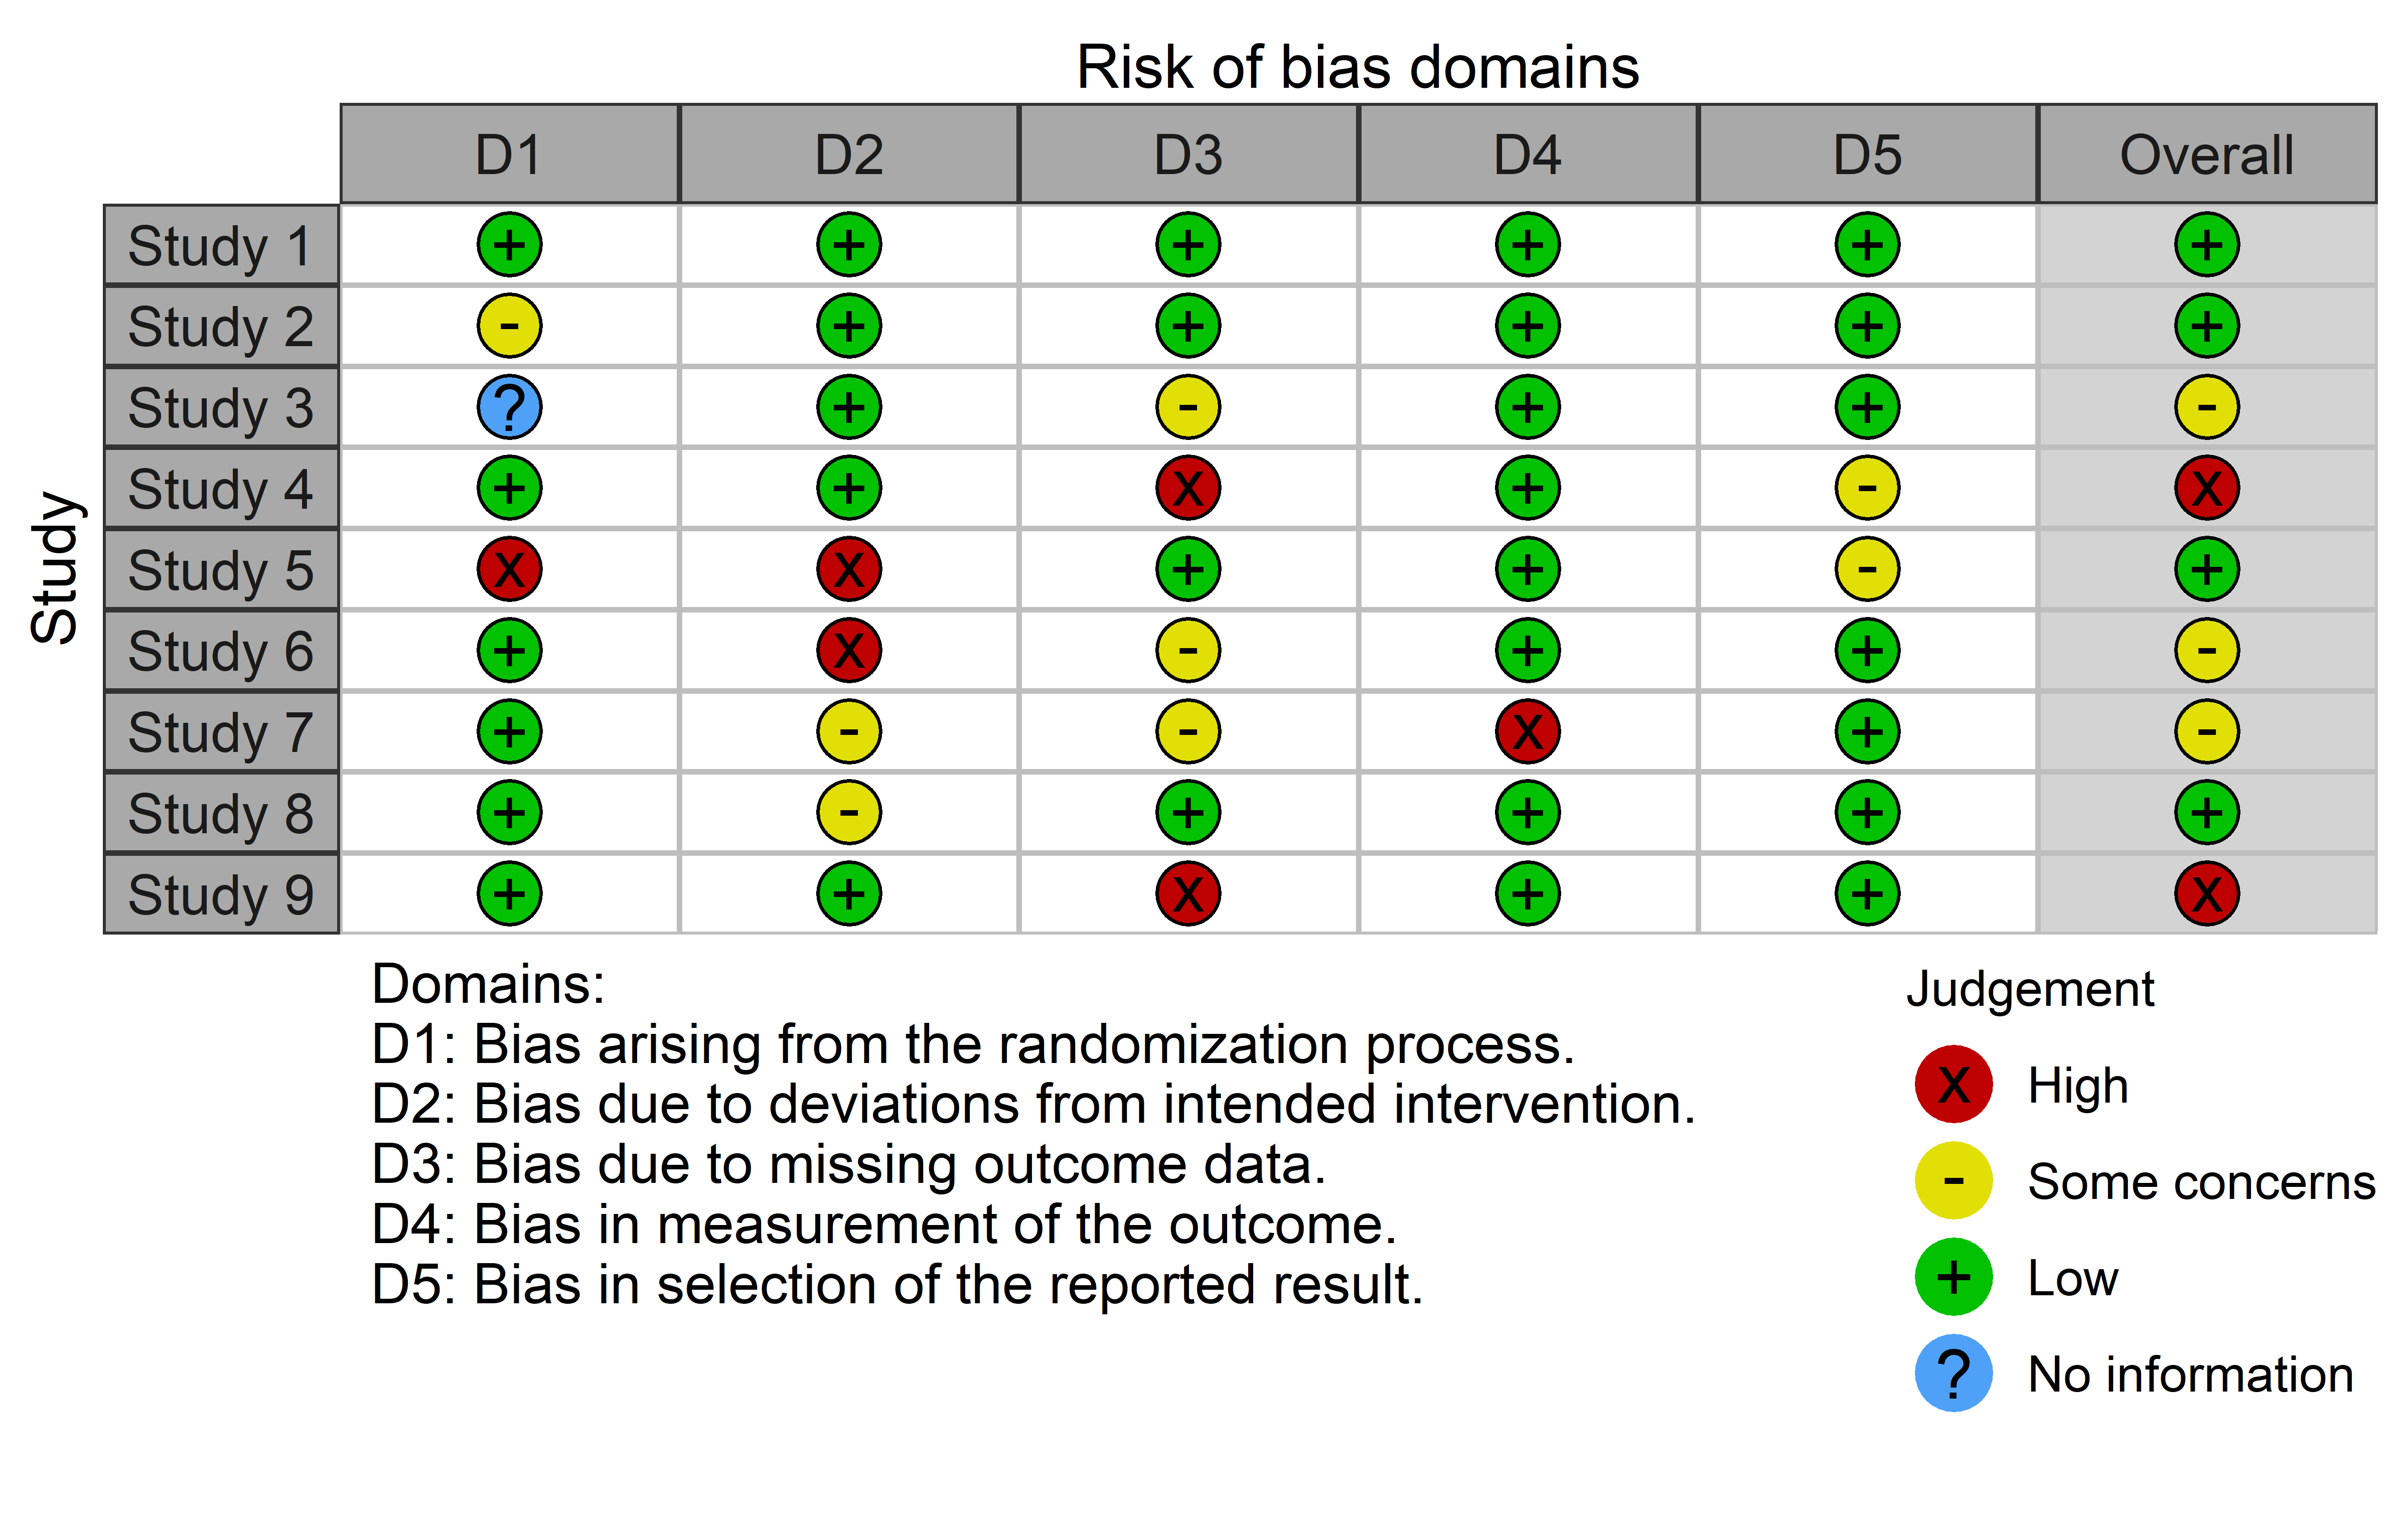
\includegraphics[width=1\linewidth]{figures/sys-rev-tools/example-rob-traffic-light-plot} \caption{Example risk of bias traffic light plot created using `robvis`}\label{fig:trafficplot}
\end{figure}

Similary, using the same data set, the summary barplot shown in Figure \ref{fig:summaryplot} is created using:

\begin{figure}
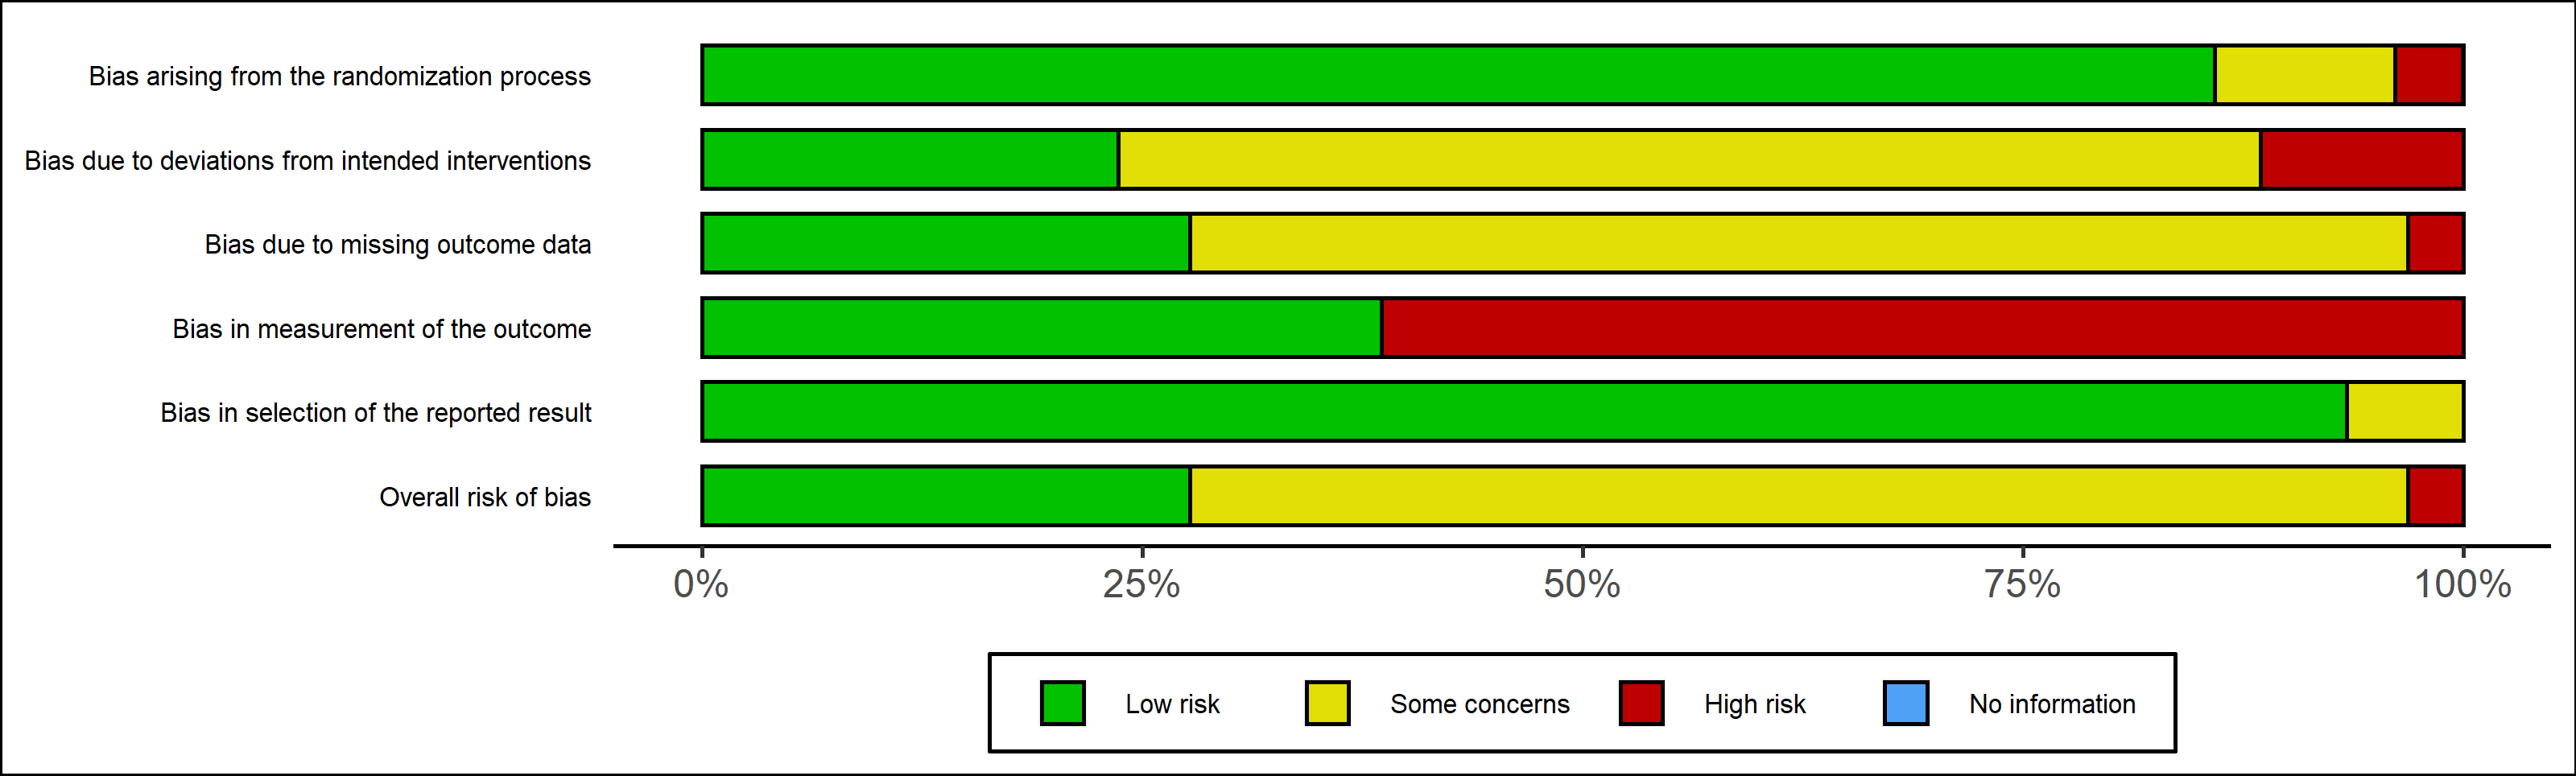
\includegraphics[width=1\linewidth]{figures/sys-rev-tools/example-rob-summary-barplot} \caption{Example risk of bias summary plot created using `robvis` and the example ROB2 dataset}\label{fig:summaryplot}
\end{figure}

A list of arguments available to the two functions in robvis are shown in Table \ref{tab:robvisarguments}

\begingroup\fontsize{9}{11}\selectfont

\begin{longtable}[t]{lcc>{\raggedright\arraybackslash}p{5cm}}
\caption{\label{tab:robvisarguments}Description of the arguments available in the two main `robvis` functions. ‘X’ indicates that the option is available for the respective function.}\\
\toprule
Argument & rob\_traffic\_light() & rob\_summary() & Description\\
\midrule
\endfirsthead
\caption[]{\label{tab:robvisarguments}Description of the arguments available in the two main `robvis` functions. ‘X’ indicates that the option is available for the respective function. \textit{(continued)}}\\
\toprule
Argument & rob\_traffic\_light() & rob\_summary() & Description\\
\midrule
\endhead

\endfoot
\bottomrule
\endlastfoot
\cellcolor{gray!6}{data} & \cellcolor{gray!6}{X} & \cellcolor{gray!6}{X} & \cellcolor{gray!6}{Defines the dataframe containing the summary (domain) level risk-of-bias assessments. See the text and Table 1 for the format expected by `robvis`}\\
tool & X & X & Defines the risk of bias assessment tool used. The RoB2 (`tool="ROB2"`), ROBINS-I (`tool="ROBINS-I"`), and QUADAS-2 (`tool="QUADAS-2"`) assessments tools are currently supported. Other tools can be visualised using the generic template (`tool = "Generic"`)\\
\cellcolor{gray!6}{colour} & \cellcolor{gray!6}{X} & \cellcolor{gray!6}{X} & \cellcolor{gray!6}{Defines the colour scheme for the plot. The default is `colour = "cochrane"` which uses the "Cochrane" (red, yellow, green) colours, while a preset option for a colour-blind friendly palette is also available (`colour = "colourblind"`). Alternatively, users can specify their own colour scheme e.g. `colour = c("\#f442c8", "\#bef441", "\#000000")`}\\
overall &  & X & Defines whether to include an additional bar showing the distibution of overall risk of bias judgements in the summary barplot figure. Default is `overall = FALSE`.\\
\cellcolor{gray!6}{weighted} & \cellcolor{gray!6}{} & \cellcolor{gray!6}{X} & \cellcolor{gray!6}{Defines whether weights should be used to produce the summary barplot figure. Default is `weighted = TRUE`, in line with current Cochrane Collaboration guidance.}\\
\addlinespace
psize & X &  & Defines the size of the points in the traffic light plot. Default is `psize = 20`.\\*
\end{longtable}
\endgroup{}

\hypertarget{reception-and-future-plans-1}{%
\subsection{Reception and Future Plans}\label{reception-and-future-plans-1}}

As of March 2021, \texttt{robvis} has been downloaded more than 10600 times. It has been well received but the systematic review community, and has been cited frequently in the published literature. A paper describing the tool was published in a special issue of Research Synthesis Methods focusing on data visualisation methods. A chapter on the tool has been incorporated in to the ``Doing Meta-Analysis in R'' online textbook.\textsuperscript{\protect\hyperlink{ref-mathias_harrer_2019_2551803}{97}}

While \texttt{robvis} is a stable package, a range of additional functionality could be added. At present, the number of tools with a specific template included in \texttt{robvis} is limited - adding additional templates is a priority. For example, a template for ROBIS, a tool for assessing risk of bias in systematic reviews, is in developement.\textsuperscript{\protect\hyperlink{ref-whiting2016robis}{98}} Additionally, the tool does not yet allow for the production of paired forest plots, where the risk-of-bias judgement is presented alongside each specific result included in the meta-analysis.\textsuperscript{\protect\hyperlink{ref-cochranechpt7}{80}} This was initially considered to be beyond the scope of the tool, as it involves the visualization of something other than risk-of-bias assessments. However, following user-driven demand, this functionality is in development and will be available in the near future. Finally, we would like to add similar functionality to that provided by the \texttt{metafor::reporter()} function, which generates a brief paragraph of text describing the results of a meta-analysis. The future \texttt{robvis::reporter()} function would provide a boilerplate description of the assessment tool used and the key domains at risk of bias.

%%%%% REFERENCES

\setlength{\baselineskip}{0pt} % JEM: Single-space References

{\renewcommand*\MakeUppercase[1]{#1}%
\printbibliography[heading=bibintoc,title={\bibtitle}]}

\end{document}
